\documentclass[a4paper, 11pt]{report}
\usepackage[pdftex]{graphicx}
\usepackage[autostyle]{csquotes}
\usepackage[backend=bibtex,style=numeric,sorting=none]{biblatex}
\usepackage{hyperref}
\usepackage{tabularx}
\usepackage{caption}
\usepackage{subcaption}
\usepackage{array}
\usepackage{amsmath}
%\usepackage{amsthm}
\newcolumntype{L}[1]{>{\raggedright\let\newline\\\arraybackslash\hspace{0pt}}m{#1}}
\newcolumntype{C}[1]{>{\centering\let\newline\\\arraybackslash\hspace{0pt}}m{#1}}
\newcolumntype{R}[1]{>{\raggedleft\let\newline\\\arraybackslash\hspace{0pt}}m{#1}}

%\theoremstyle{definition}
%\newtheorem{exmp}{Example}[section]

\addbibresource{bibliography}

\begin{document}

\pagenumbering{roman}
\begin{titlepage}
\begin{center}

{\Huge \bfseries
Optimizing Cycle Shrinking Algorithm for Constant Dependence Distances\\
}~\\[1cm]

% The '~' is needed because \\ only works if a paragraph has started.

{\large

}~\\[0.20cm]

{\Large \bfseries
B. Tech Project Report
}\\[2.75cm]

{\Large \bfseries
Sameep Bagadia\\
Roll no: 100050003\\

~\\
under the guidance of Prof. Supratim Biswas
}~\\[1cm]

\vfill


\includegraphics[width=6cm]{Figures/logo.png}~\\[1cm]

{\large \bfseries
Department of Computer Science and Engineering\\
Indian Institute of Technology Bombay\\
}

\end{center}
\end{titlepage}
\chapter*{Abstract}
In this report we present an optimal algorithm for cycle shrinking transformation for parallelizing compilers. We first give a motivation for a better algorithm by pointing out that the extended cycle shrinking algorithm is not optimal when there is no dominating dependence distance. Then we give our algorithm to generate the partitions in the iteration space of loops in constant dependence distance case. We prove the correctness and optimality of our approach. We also give a method to calculate the number of partitions that our algorithm will generate without actually creating the partitions. We then proceed to give an algorithm to generate loops from the partitions we created. We also prove the correctness of this algorithm. Then we consider the variable dependence distance case and give a better algorithm than extended cycle shrinking algorithm. We also prove that the number of partitions generated by our algorithm is optimal. We also give some ideas for parallelizing our algorithm.
\addcontentsline{toc}{chapter}{Abstract}
%\chapter*{Acknowledgements}
Acknowledgements should be simple, in good taste, and fit on one page.
\addcontentsline{toc}{chapter}{Acknowledgements}
%\chapter*{Honor Code}
We certify that we have properly cited any material taken from other sources and have obtained permission for any copyrighted material included in this report. We take full responsibility for any code submitted as part of this  project and the contents of this report.\\
% This space is for putting the signatures.
\vspace*{15mm}

\begin{flushright}
Author-1 (Entry No.)\\
\end{flushright}

\vspace*{15mm}

\begin{flushright}
Author-2 (Entry No.)\\
\end{flushright}

\vspace*{15mm}

\begin{flushright}
Author-3 (Entry No.)\\
\end{flushright}

\addcontentsline{toc}{chapter}{Honor Code}
%\chapter*{Certificate}
It is certified that the B. Tech. project ``Title Of The Project" has been done by students: Author-1 (Entry No.), Author-2 (Entry No.) and Author-3 (Entry No.) under my supervision. This report has been submitted towards partial fulfillment of B. Tech. degree requirements. \\
% This space is for putting the signatures.
\vspace*{15mm}

\begin{flushright}
Supervisor's Name \\
Faculty Supervisor \\
Designation, Department of Computer Science and Engineering \\
Indian Institute of Technology Ropar \\
Rupnagar-140001, Punjab, India \\
\end{flushright}

\vspace*{15mm}

% This is not needed for some projects.
\begin{flushright}
Supervisor's Name \\
Industry Supervisor \\
Designation, Company's Name \\
Address Line - 1 \\
Address Line - 2 \\
\end{flushright}

\addcontentsline{toc}{chapter}{Certificate}
\tableofcontents
%\listoffigures
\addcontentsline{toc}{chapter}{List of Figures}
%\listoftables
\addcontentsline{toc}{chapter}{List of Tables}
%\chapter*{Nomenclature}
\addcontentsline{toc}{chapter}{Nomenclature}
\pagenumbering{arabic}
\chapter{Introduction}


A parallelizing compiler converts a sequential program to a semantically equivalent parallel program. For this transformation to be correct, data dependences must be satisfied. Therefore, data dependence analysis is done. There are various tests for data dependence like GCD test, Banerjee test, Delta test etc.~\cite{allenoptimizing}\\

A data dependence graph (DDG) is a directed graph with each statement as a vertex and an edge from statement $S_i$ to $S_j$ if there is a dependence $S_i \delta S_j$. \\

Based on the DDG, transformations are applied to the sequential code. There are many transformations like loop fusion, loop skewing, loop interchange etc.~\cite{allenoptimizing}. But most of these transformations work only when the data dependences do not form a cycle. In the case when there is a cyclic dependence straightforward parallelization cannot be done. In such cases, cycle shrinking algorithm can be used.\\


\chapter{Literature Survey}
\section{Cycle Shrinking Algorithm}

Cycle shrinking algorithm~\cite{cycle1} allows loops with cyclic data dependencies to be partially parallelized when the dependence distances are known. Minimum distance between source and sink for a dependence is known as dependence distance. This is a vector for nested loops. \\

The idea of cycle shrinking has been extended in three ways: \\
\begin{enumerate}
\item {\bf Simple shrinking}: Minimum dependence distance for each nest level is calculated separately and then partitions are created based in these values. 
\item {\bf Selective shrinking}: Outermost level with positive dependence distance is selected and then simple shrinking is applied only at this level. All lower level loops are done in parallel. 
\item {\bf True distance shrinking}: The partition is made based on the actual number of iterations between the source and the sink ("true distance") of the dependencies considering the loop bounds at each nest level. 
\end{enumerate}

\subsection{Example}
Consider the following example: \\
DO I = 0 to 9 \\
\indent DO J = 0 to 9 \\
\indent \indent A[I+3, J+4] = B[I, J] \\
\indent \indent B[I+2, J+3] = A[I, J] \\
\indent ENDO \\
ENDO \\

The two dependence distances are (3, 4) and (2, 3). The partitions created by cycle shrinking algorithm are shown in the figure~\ref{fig:cycle_shrinking_example}. \\


\begin{figure}
\centering
\begin{subfigure}{0.45\textwidth}
  \centering
  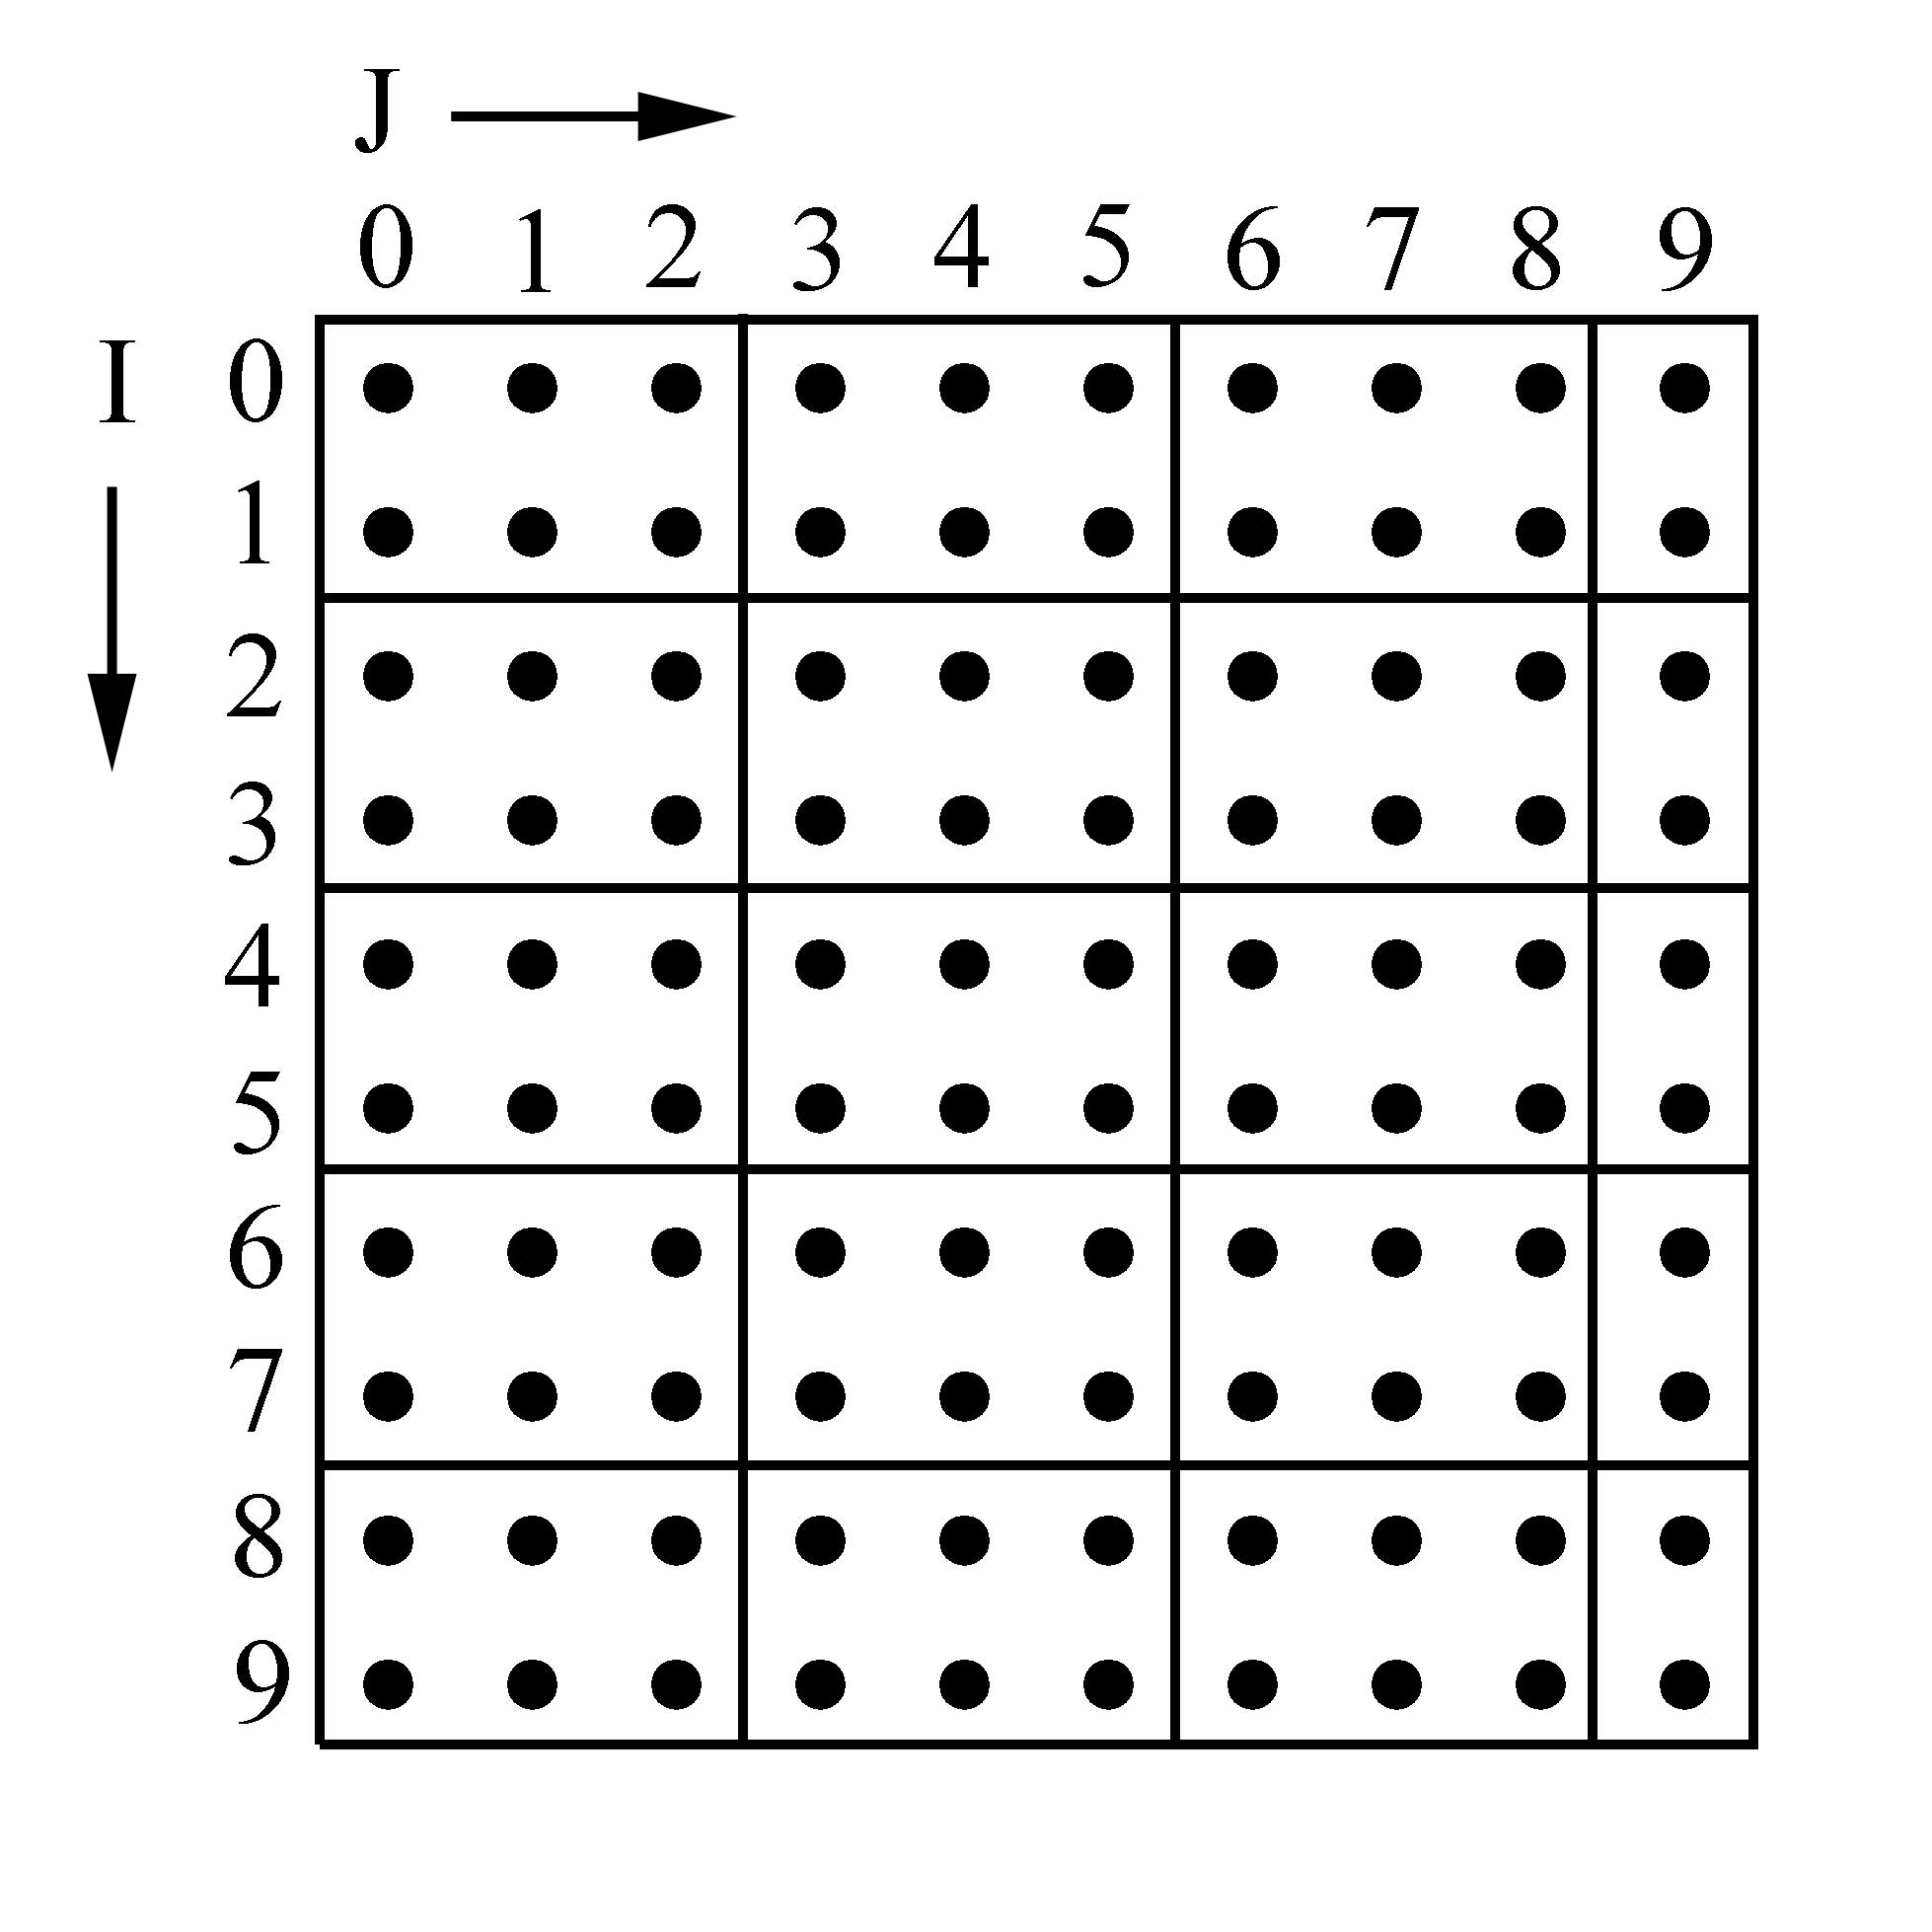
\includegraphics[width=\textwidth]{Figures/simple.jpg}
  \caption{}
  \label{fig:simple}
\end{subfigure} 
\begin{subfigure}{0.45\textwidth}
  \centering
  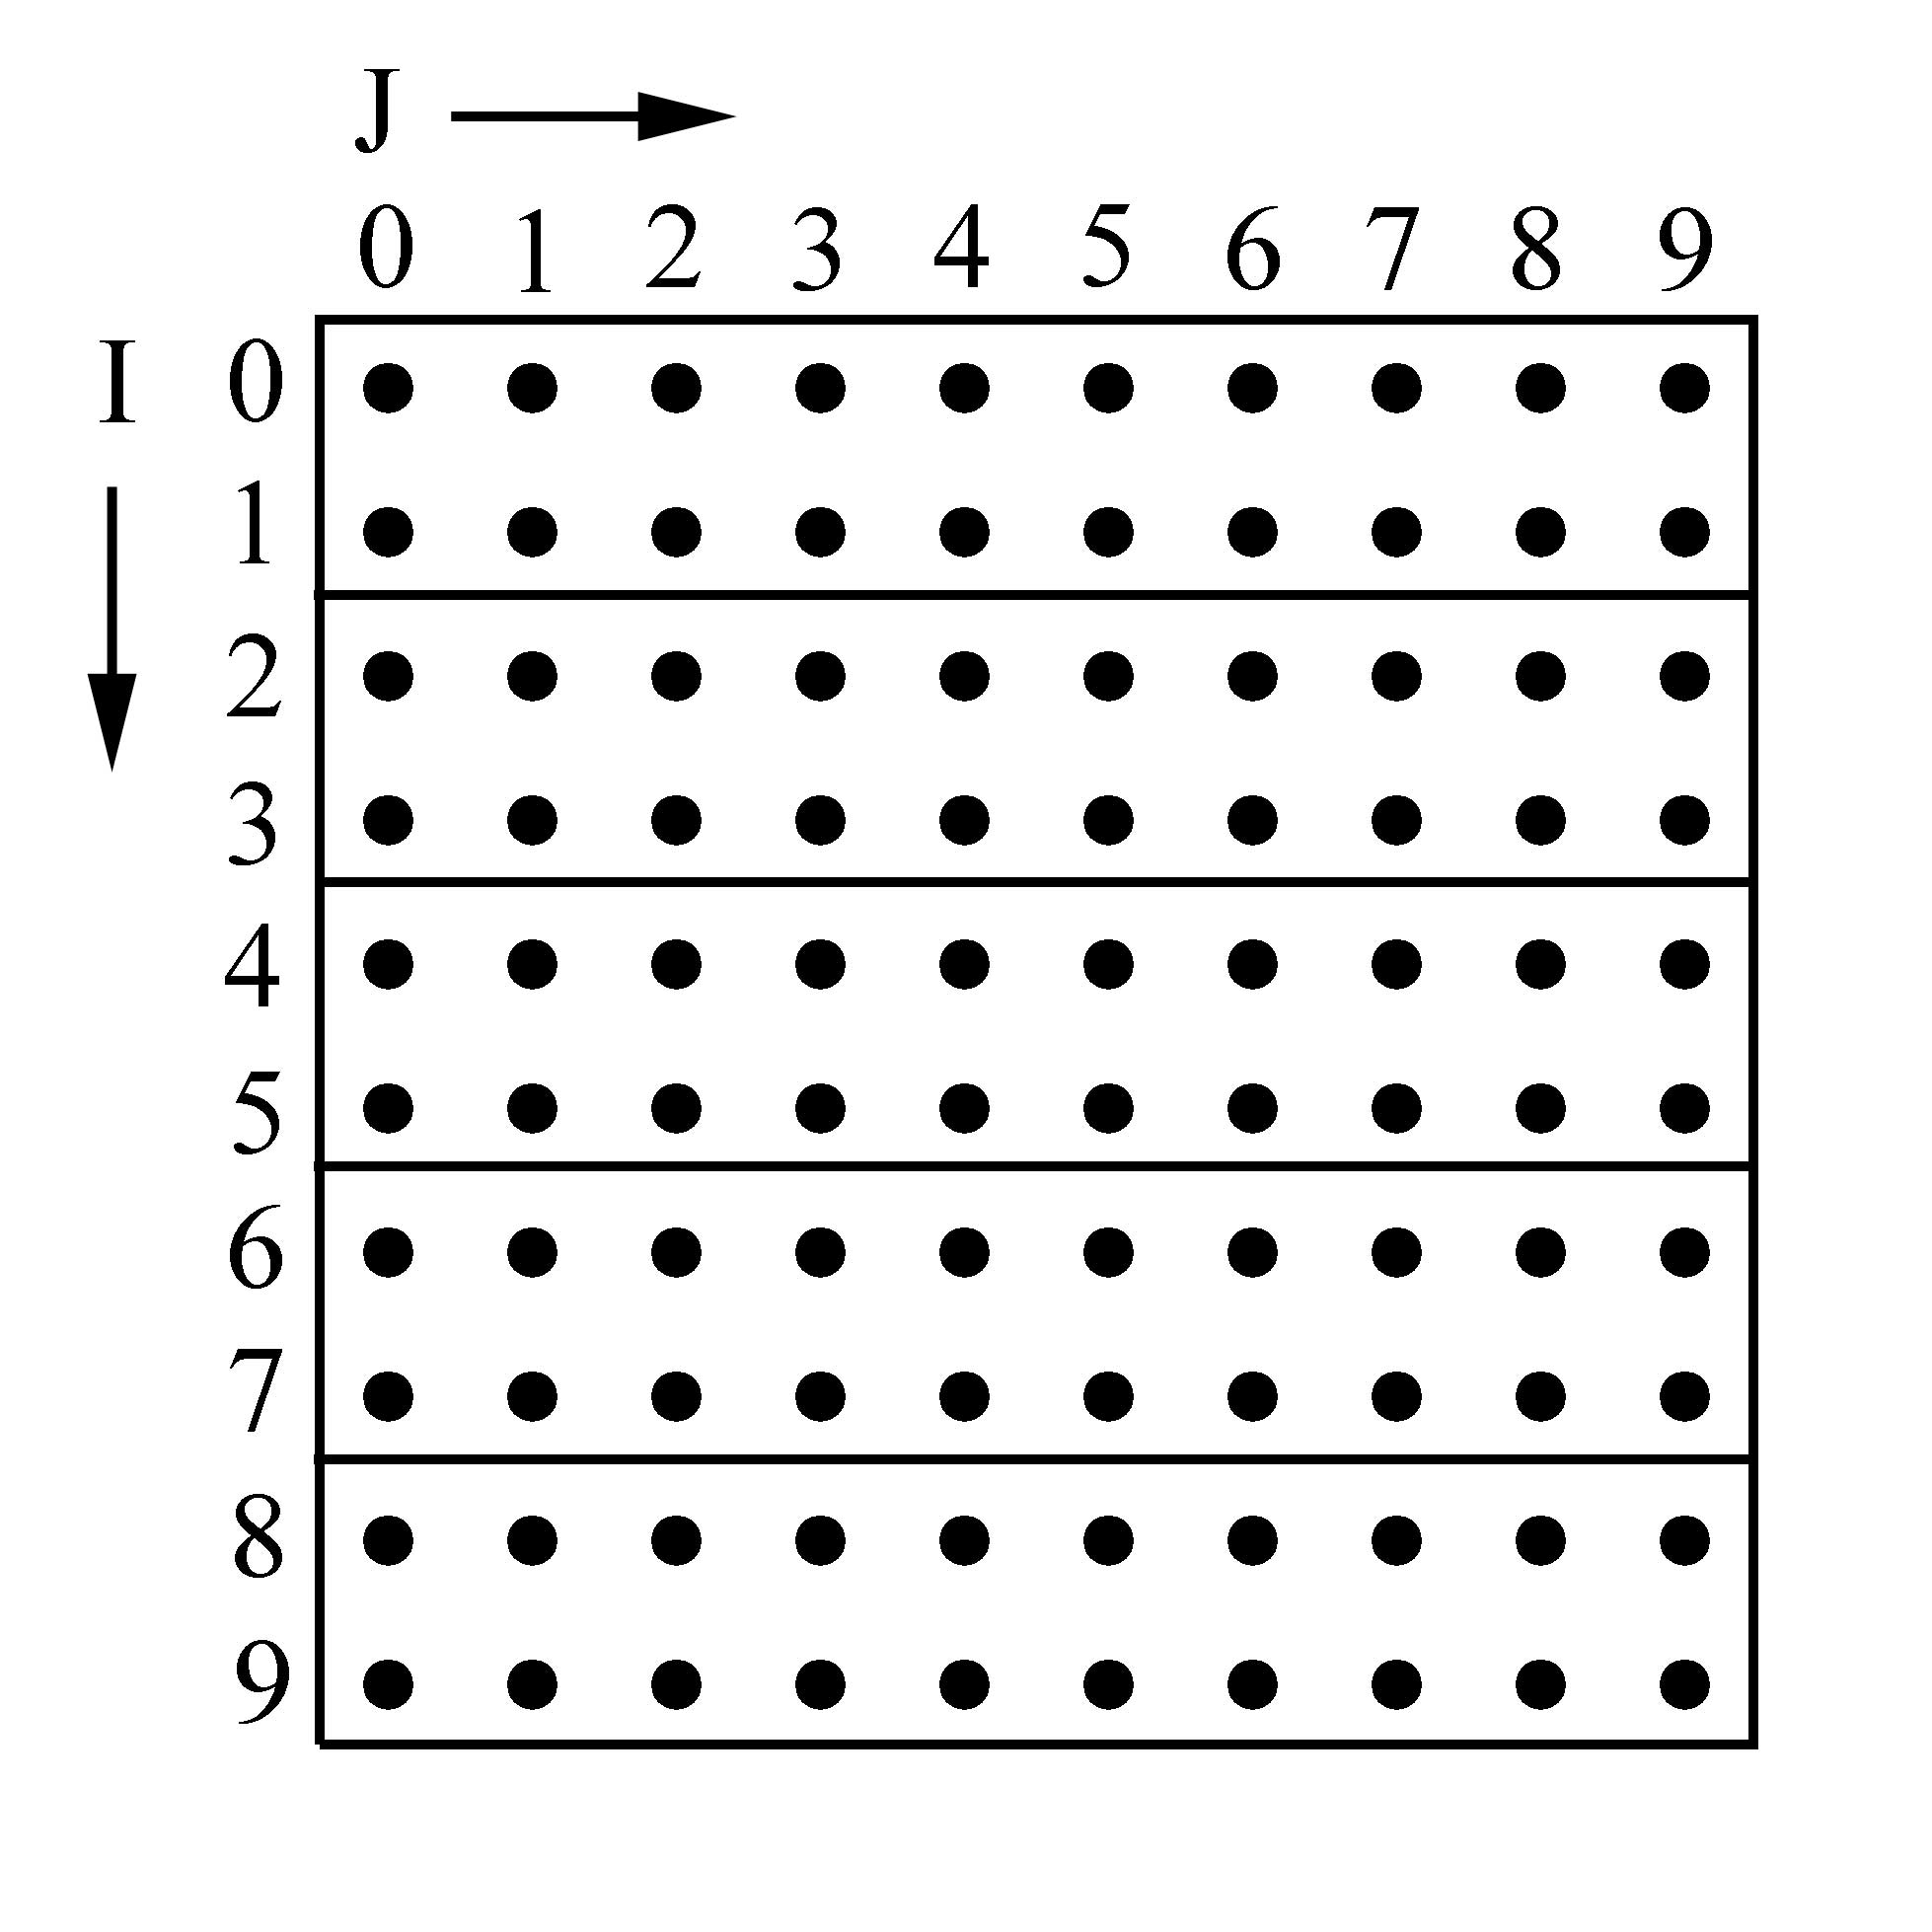
\includegraphics[width=\textwidth]{Figures/selective.jpg}
  \caption{}
  \label{fig:selective}
\end{subfigure}  \\
\begin{subfigure}{0.45\textwidth}
  \centering
  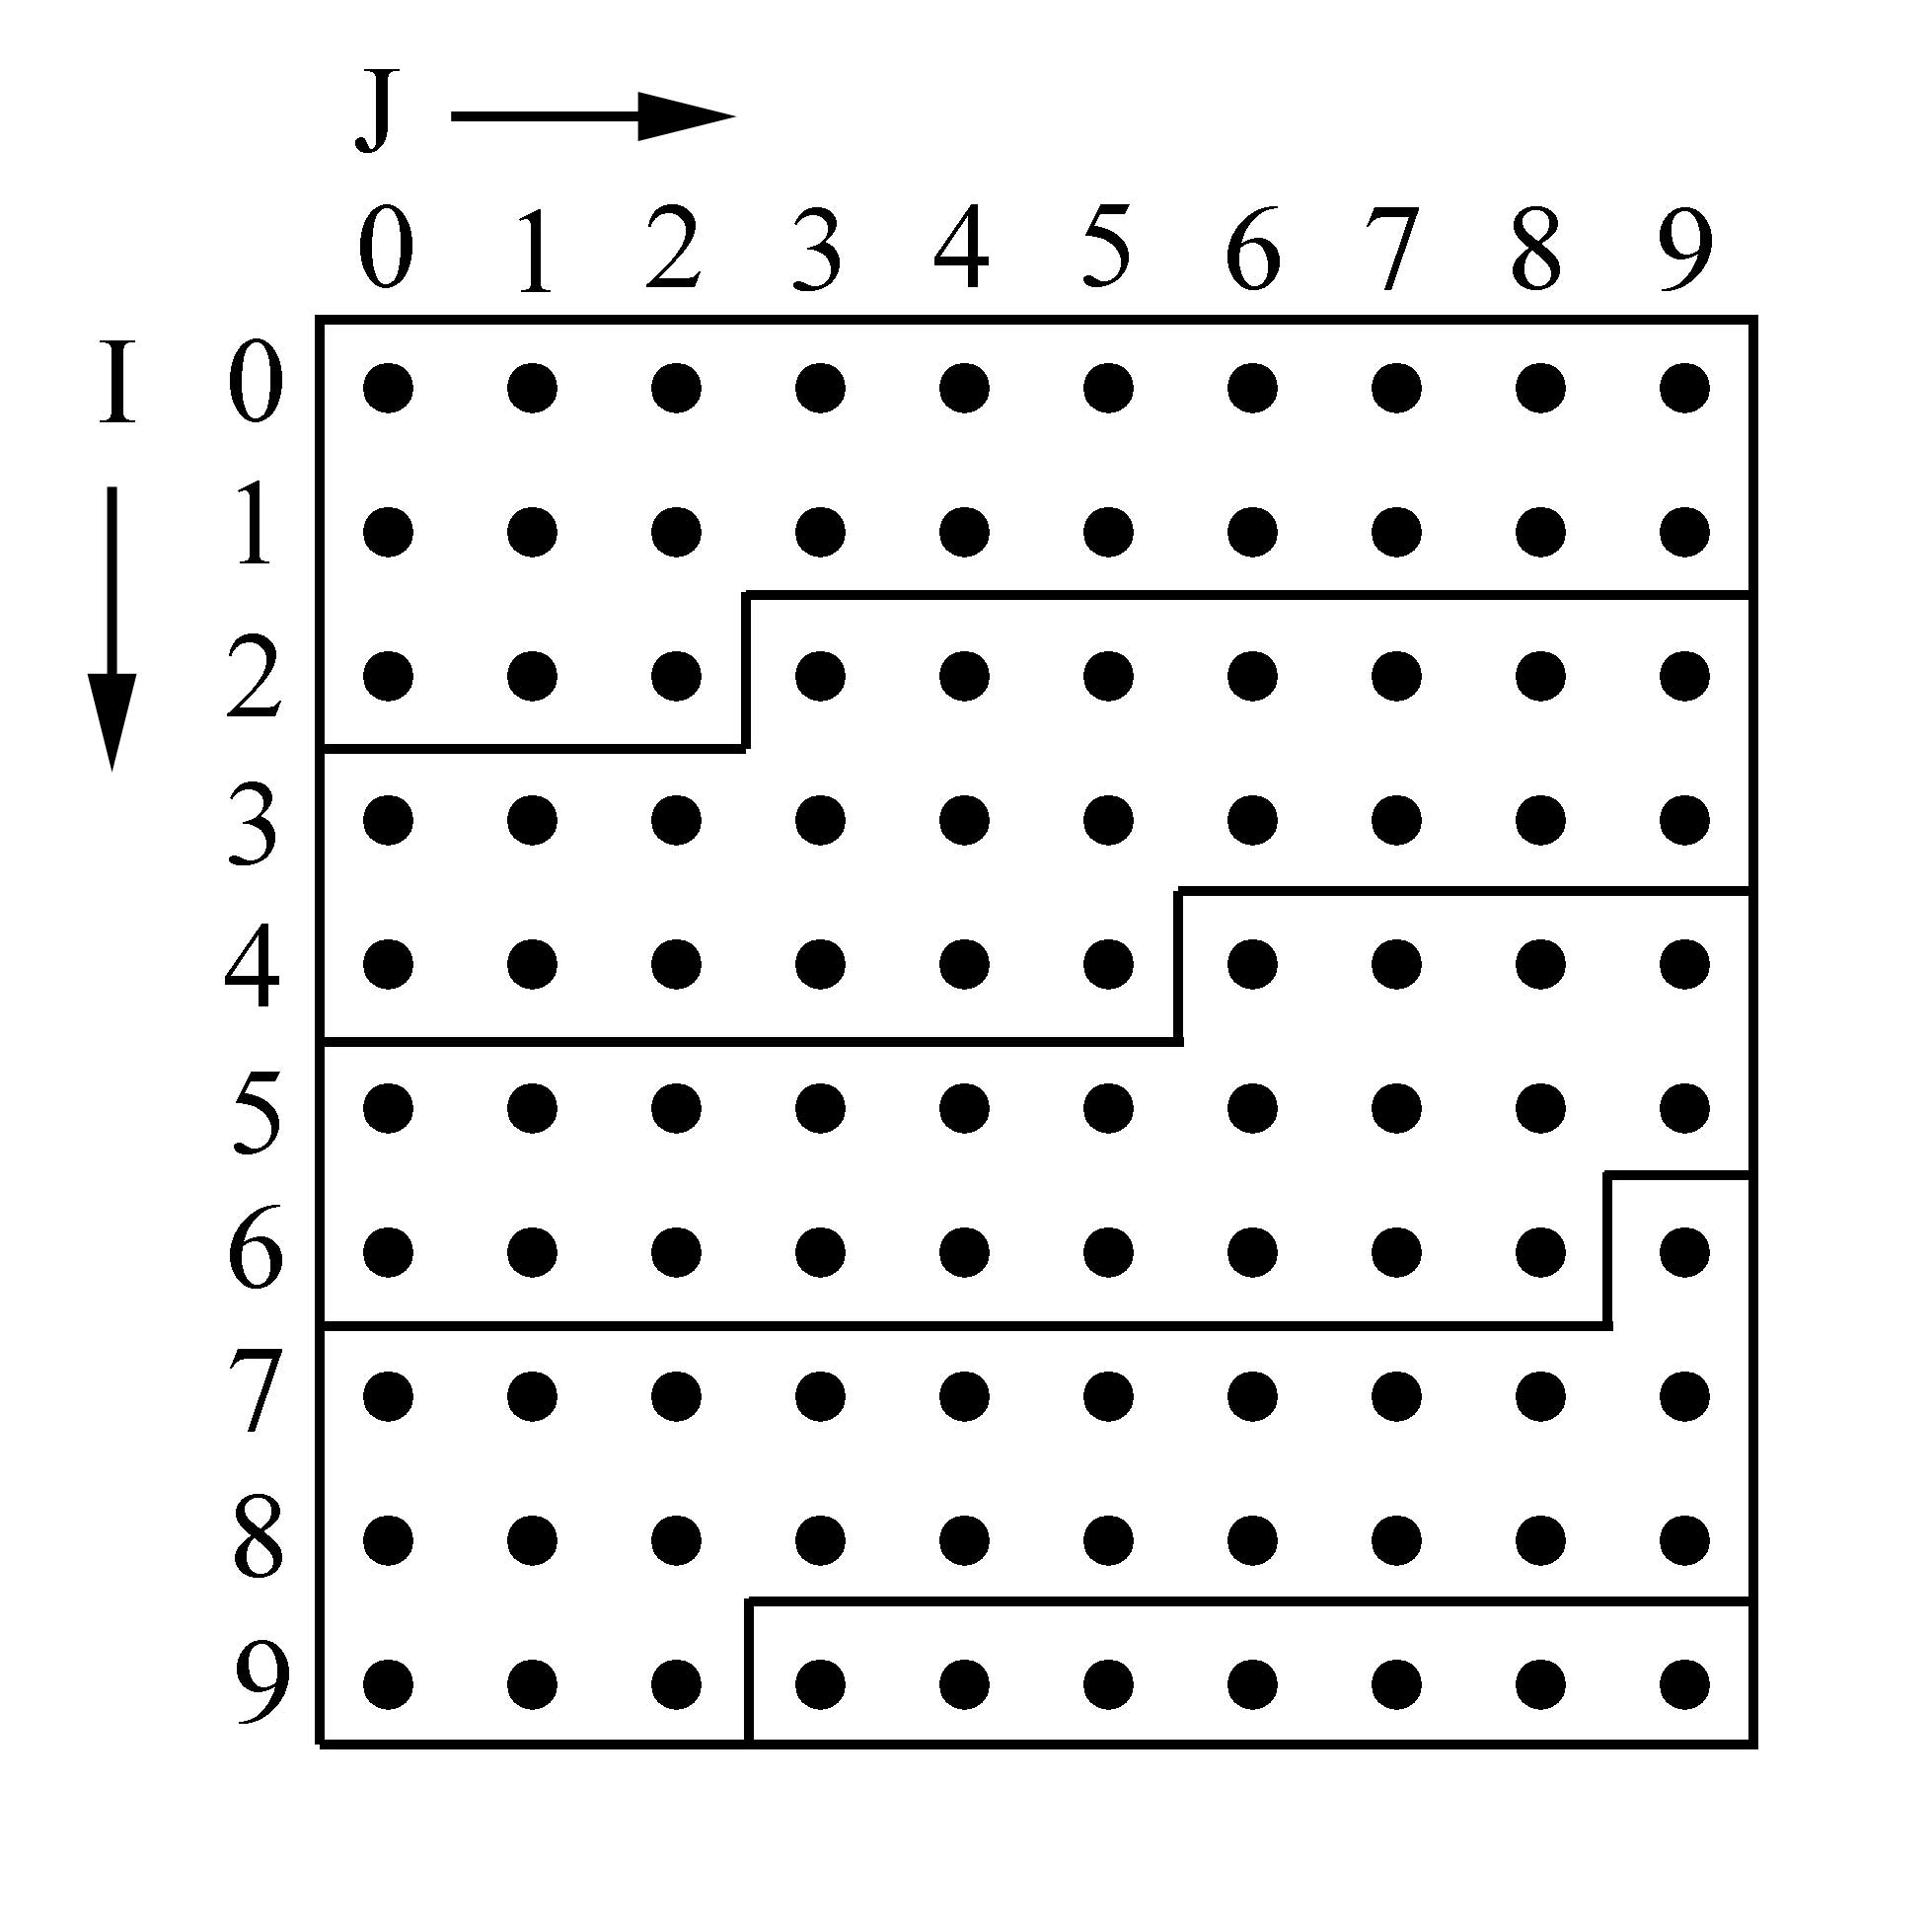
\includegraphics[width=\textwidth]{Figures/true_distance.jpg}
  \caption{}
  \label{fig:true_distance}
\end{subfigure}
\begin{subfigure}{0.45\textwidth}
  \centering
  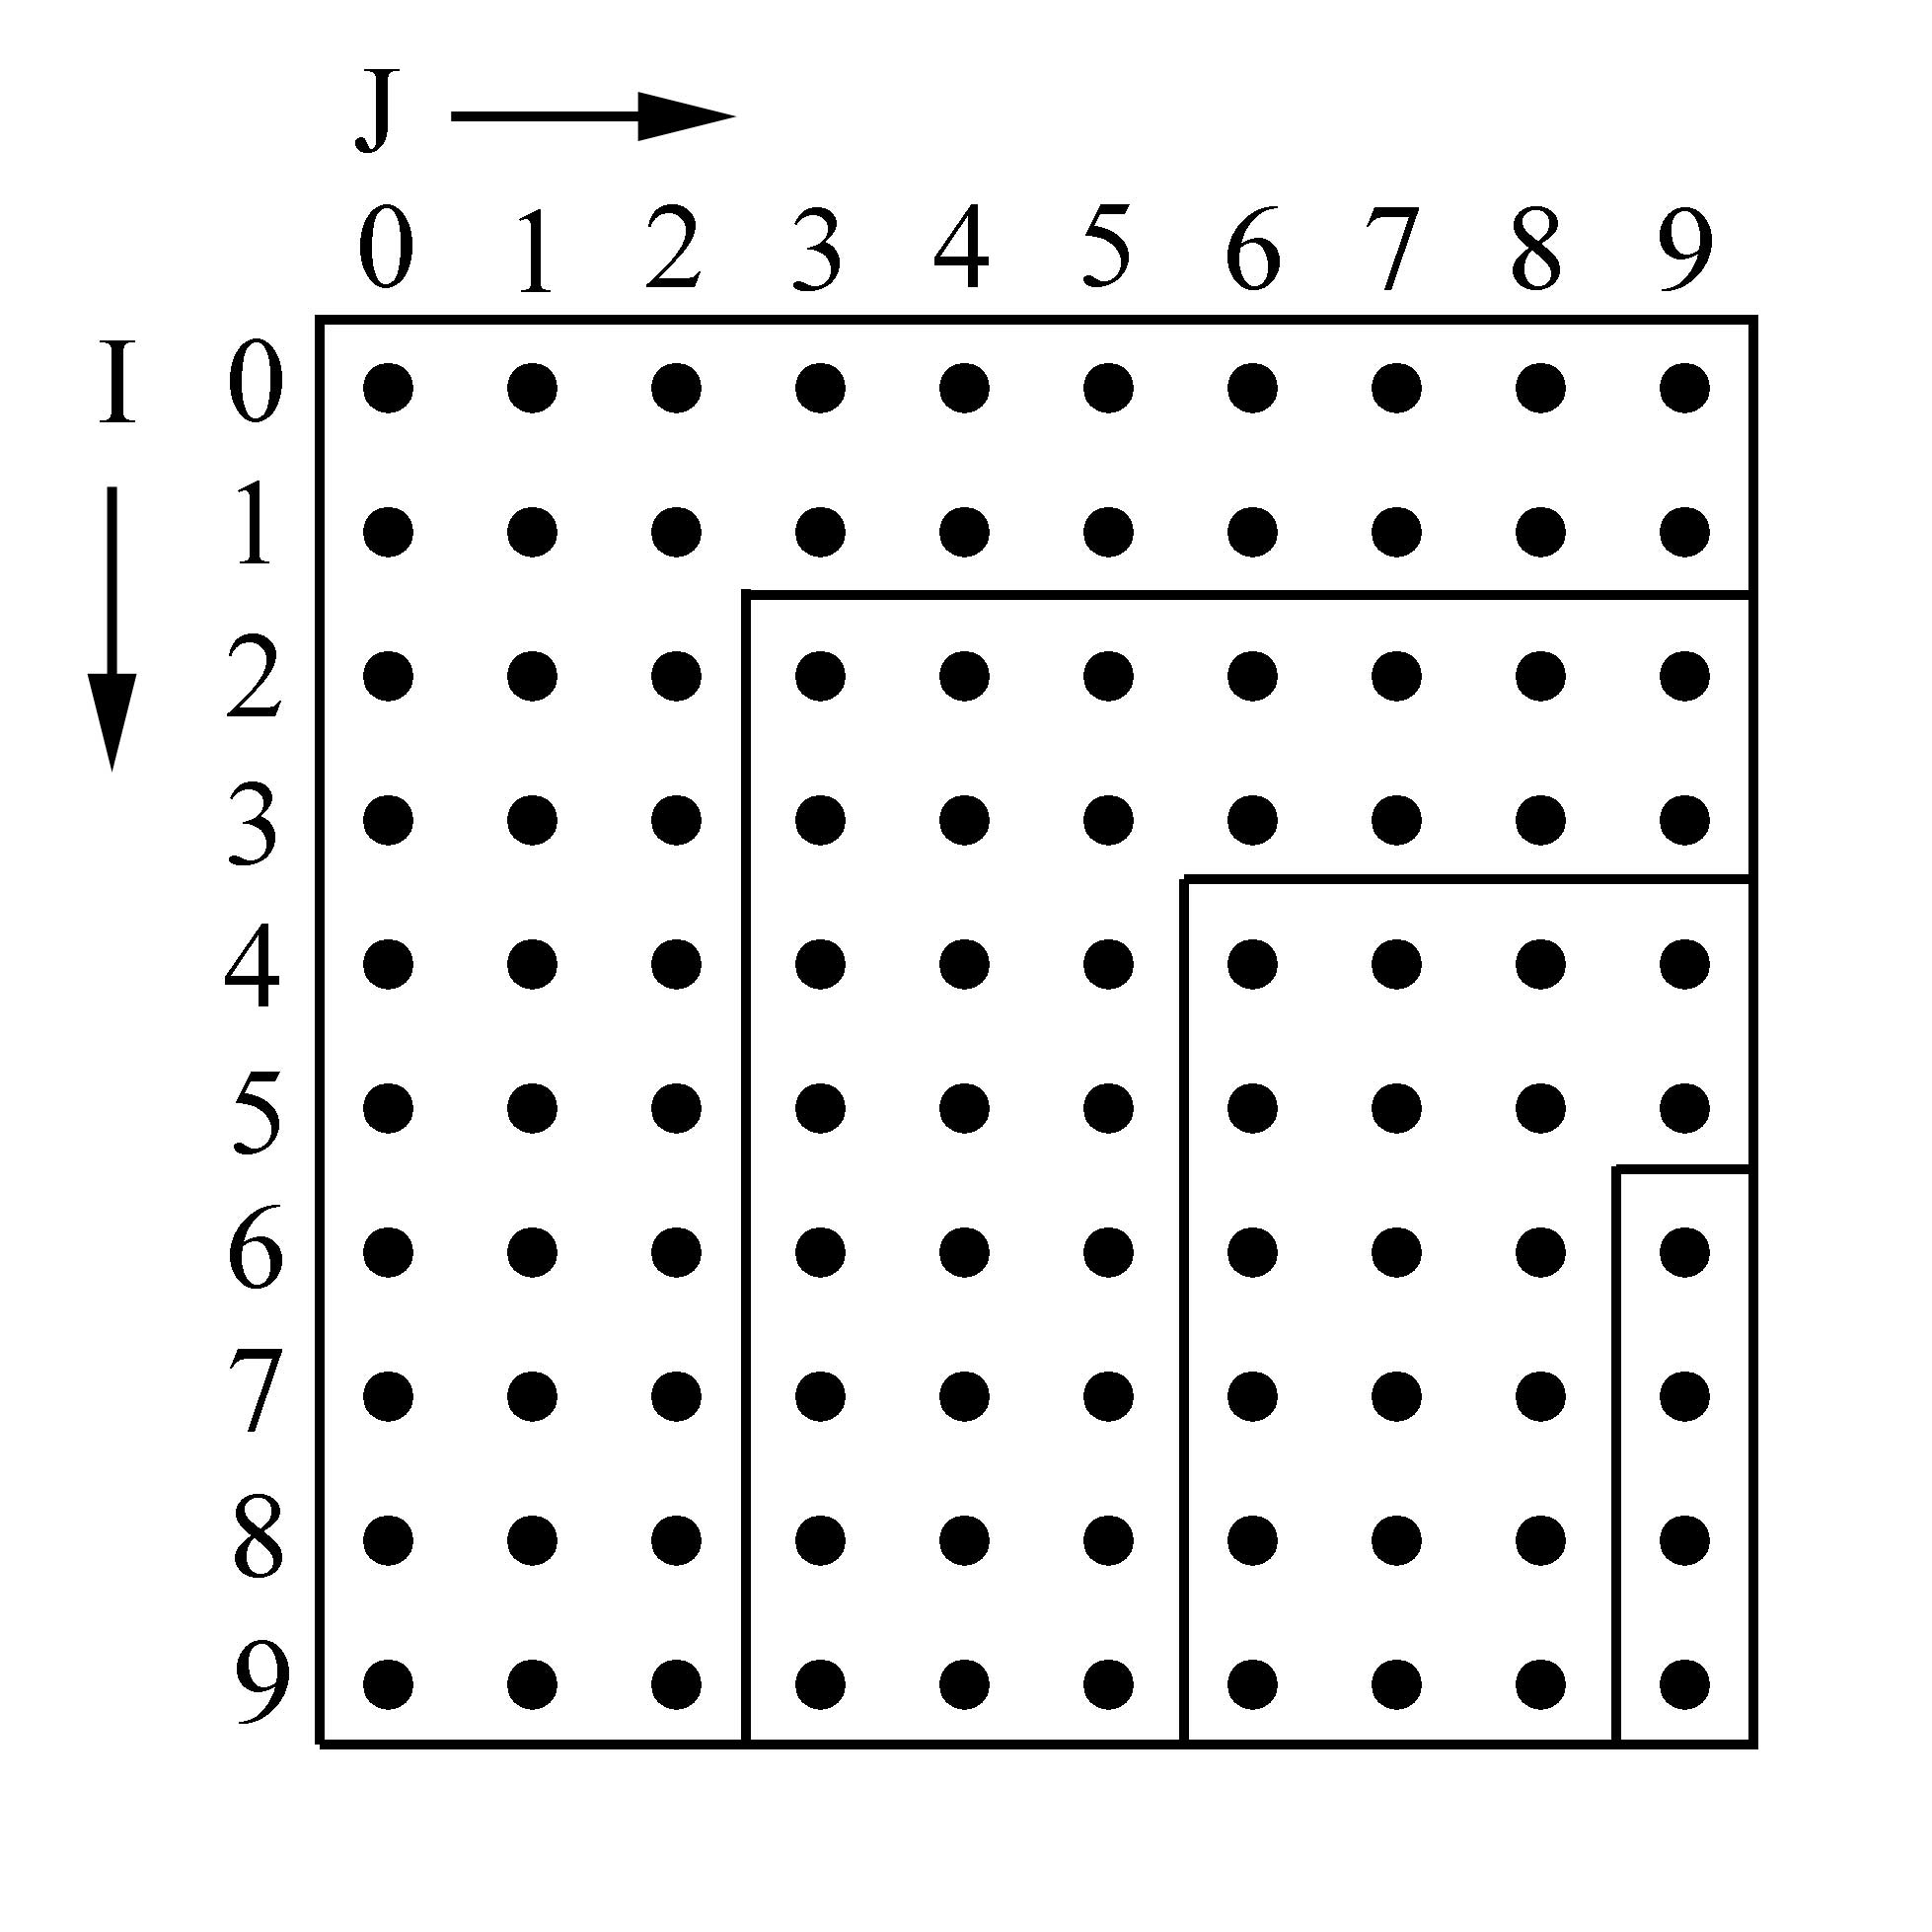
\includegraphics[width=\textwidth]{Figures/extended.jpg}
  \caption{}
  \label{fig:extended}
\end{subfigure}
\caption{(a) Partitions by simple shrinking. (b) Partitions by selective shrinking. (c) Partitions by true distance shrinking. (d) Partitions by extended cycle shrinking algorithm}
\label{fig:cycle_shrinking_example}
\end{figure}

However, a greater degree of parallelism can be achieved if the partitions are made as shown in the figure~\ref{fig:extended}. It reduces the number of partitions.
Extended cycle shrinking algorithm creates paritions in this manner. \\


\section{Extended Cycle Shrinking Algorithm}

Extended Cycle Shrinking Algorithm~\cite{extended} has two cases, when there are only constant dependence distances and when there are variable dependence distances. \\

\subsection{Constant Dependence Distances}

If two array accesses have a dependence among them then they are called as a reference pair.
Consider the case where all the reference pairs have only constant dependence distances. The dependence distance vector of a reference pair R is denoted as $\Phi(R)$ and $k^{th}$ component of the dependence distance $\Phi(R)$ is denoted as $\Phi_{k}(R)$. Then we define the dependence distance of vector of loop L denoted by $\Phi(L)$ as given below: \\

For each nest k of the loop, 
\begin{itemize}
\item $\Phi_k(L) = 0$ if there exists some reference pair R for which $\Phi_k(R) = 0$, or there exist two reference pairs R and R' such that $\Phi_k(R)$ and $\Phi_k(R')$ have opposite signs. 
\item $\Phi_k(L) = min(|\Phi_k(R)|)$ if sign($\Phi_k(R)$) is positive for all R, and
\item $\Phi_k(L) = -min(|\Phi_k(R)|)$ otherwise.
\end{itemize}

The partitions are created using $\Phi(L)$. The $k^{th}$ coordinate of the $i^{th}$ apex point of the partition is $(i-1)*\Phi_k(L)$ if $\Phi_k(L) > 0$, otherwise the apex point for that index is calculated from the other end of loop bound and the direction of partition is also opposite. \\

For example of figure~\ref{fig:extended}, \\
$\Phi(L) = (2, 3)$ \\
Therefore the apex points are (0, 0), (2, 3), (4, 6) and (6, 9). \\

\subsection{Variable Dependence Distances}

In the case of variable dependence distances, only those cases are considered where each source can have only one sink for a given reference pair. Unlike in the constant dependence distance case, here the dependence distaces vary with the loop indices. Dependence distance is function of loop indices in this case. Thus, instead of summarizing the dependence for the entire loop, the summarization is done at each apex. \\

As shown in the figure~\ref{fig:variable1}, apex1 is the initial apex point. We obtain apex2' and apex2'' as sinks of apex1. Then the sinks of all sources inside the cone of apex1 lie inside the cones formed by apex2' and apex2''. We summarize these two apexes to obtain apex2 as the next apex point in the partition. This procedure is repeateed to obtain subsequent apex points. Once the apex points are known, the partitions are created in similar way as was done in the constant dependence distance case. \\

\begin{figure}
\caption{Variable dependence distances}
\label{fig:variable1}
\centering 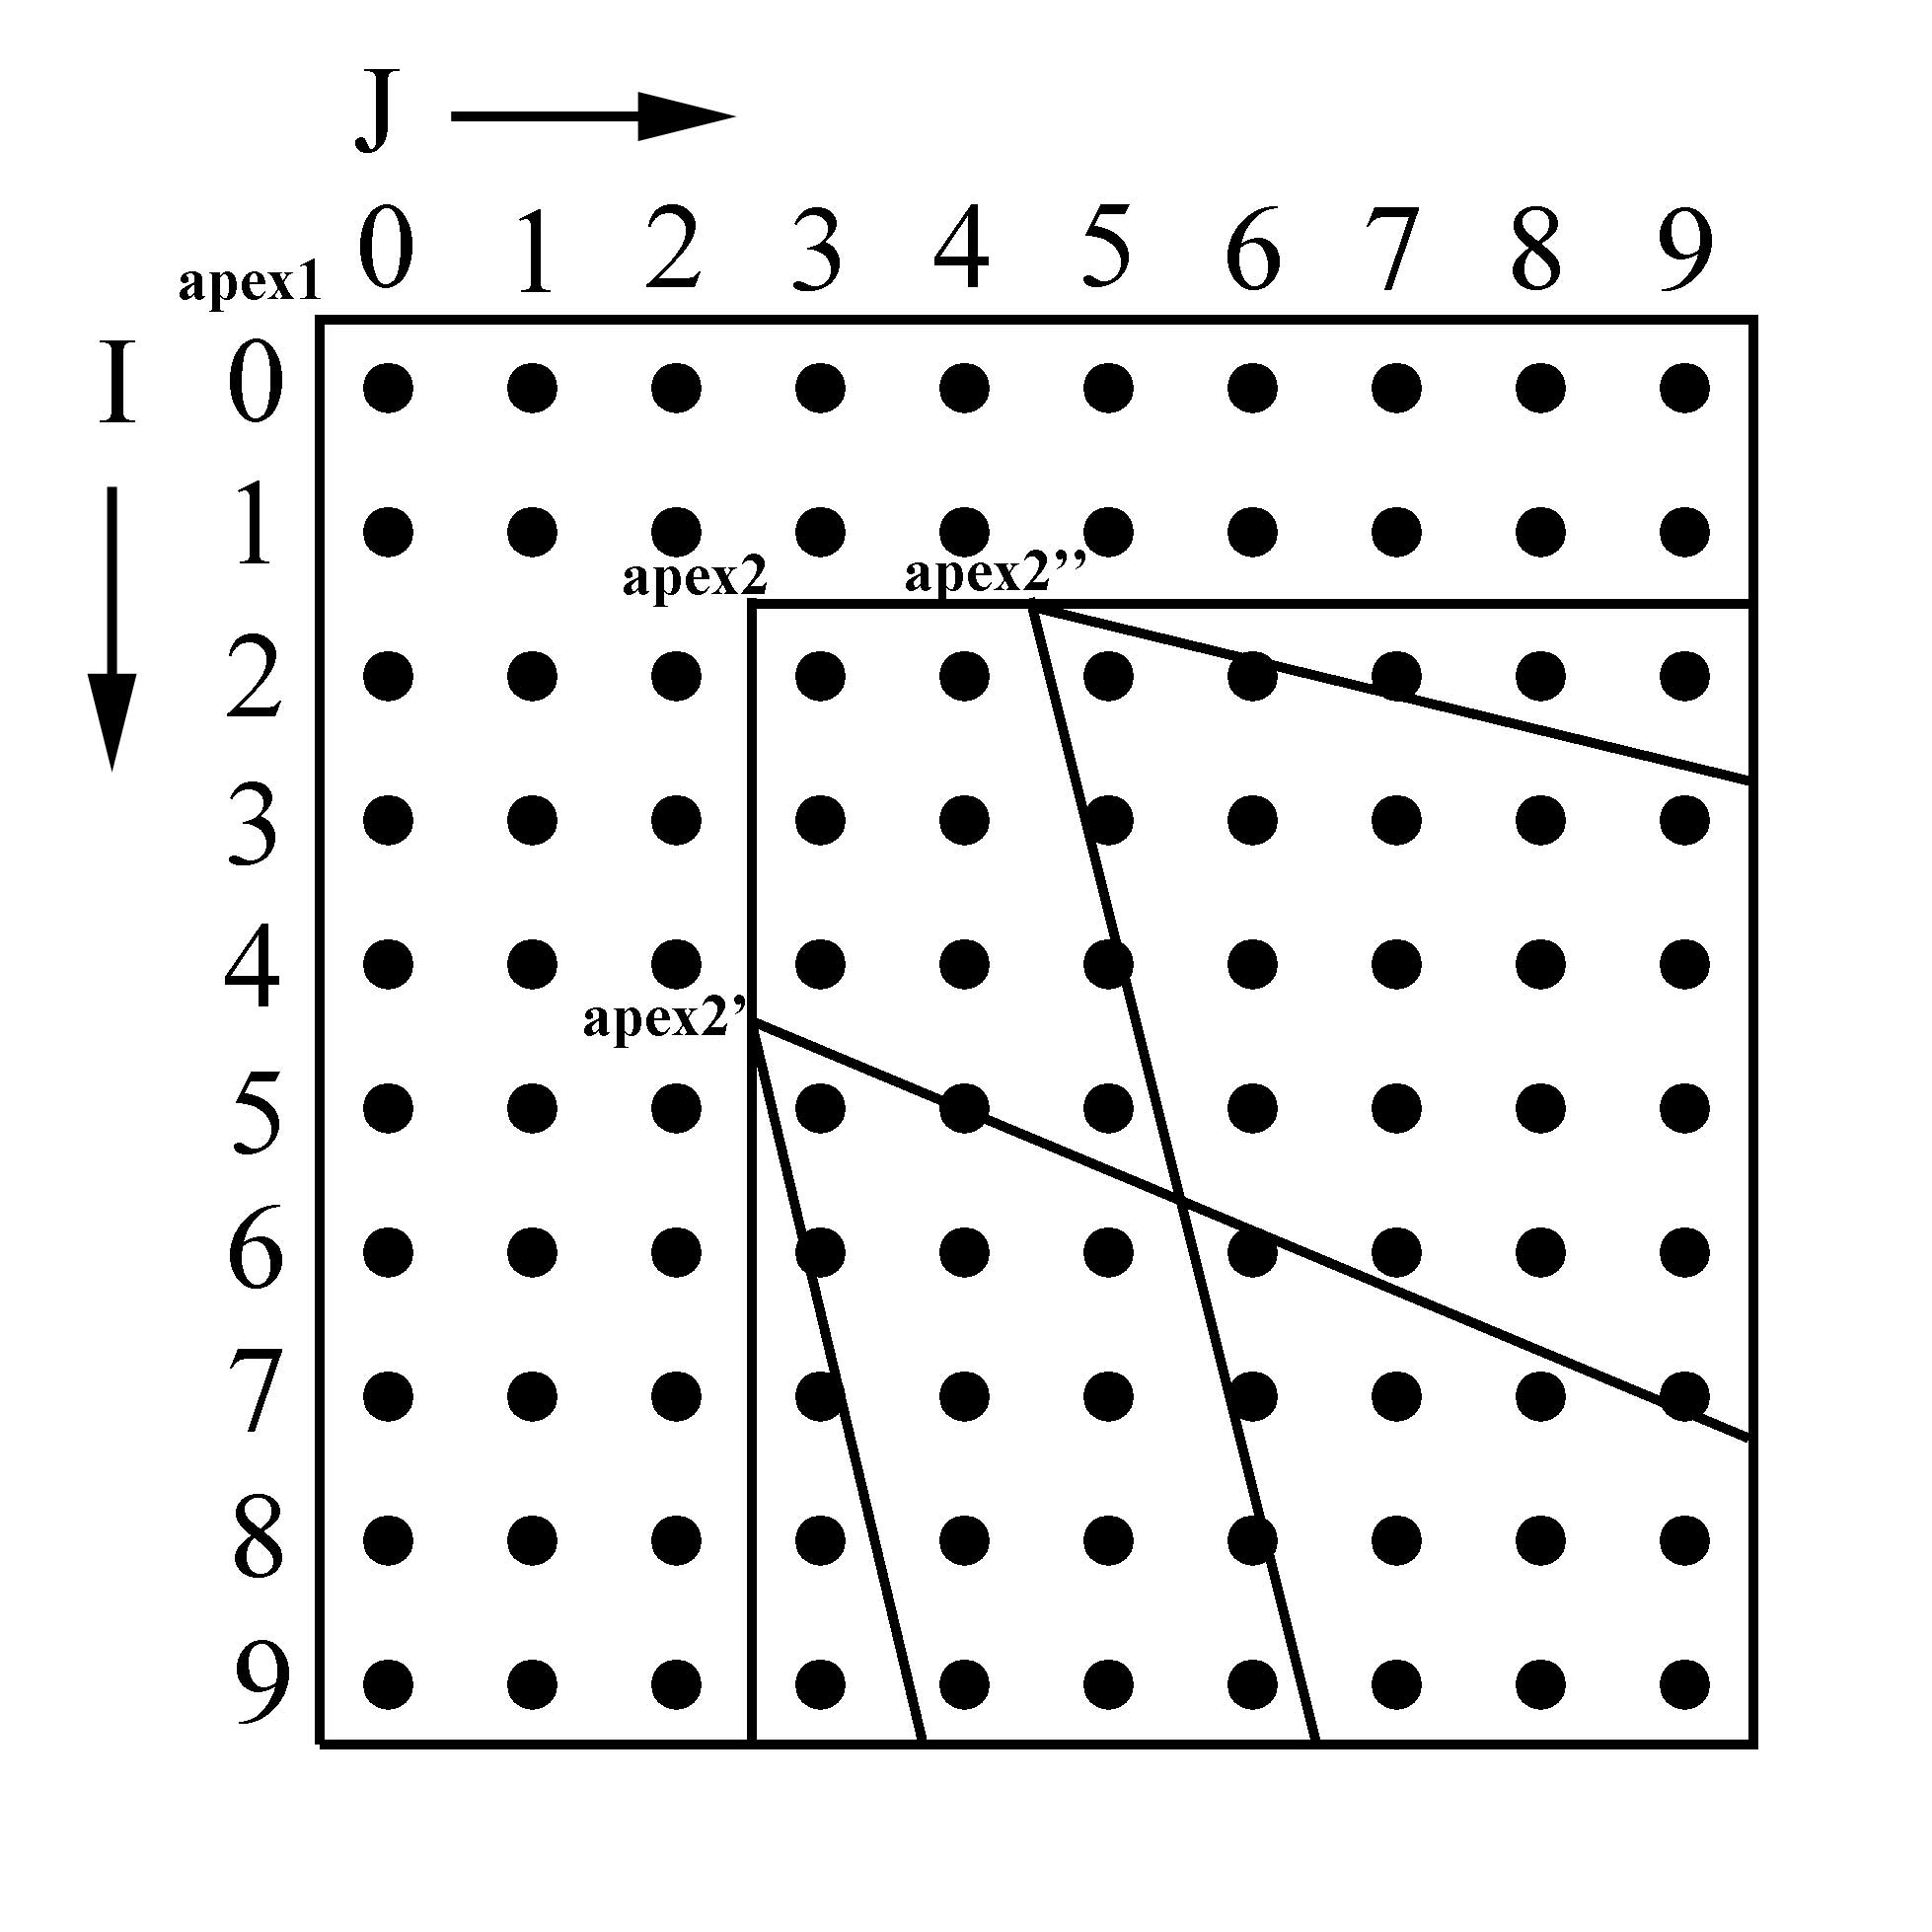
\includegraphics[width=0.5\textwidth]{Figures/variable1.jpg}
\end{figure}

\noindent Consider the following example: \\
DO I = 0 to 9 \\
\indent DO J = 0 to 9 \\
\indent \indent A[2I+J+3, I+4J+2] = B[I+3, J+3] \\
\indent \indent B[3I+J+4, 2I+2J+3] = A[I+1, J+1] \\
\indent ENDO \\
ENDO \\

\noindent Dependence distances are : \{(I+J+2, I+3J+1), (2I+J+1, 2I+J)\} \\

\noindent apex1 = (0, 0)\\
Dependence distances: \{(2, 1), (1, 0)\}\\
Summarized dependence distance = (1, 0)\\
apex2 = (1, 0)\\

\noindent Dependence distances: \{(3, 2), (3, 2)\}\\
Summarized dependence distance = (3, 2)\\
apex3 = (4, 2)\\

\noindent Dependence distances: \{(8, 11), (11, 10)\}\\
Summarized dependence distance = (8, 10)\\
apex4 = (12, 12) which is out of range and thus all partitions have been found\\

The partitions generated from this example are shown in the figure~\ref{fig:variable_eg}
\begin{figure}
\caption{Partitions created in the example of variable dependence distance}
\label{fig:variable_eg}
\centering 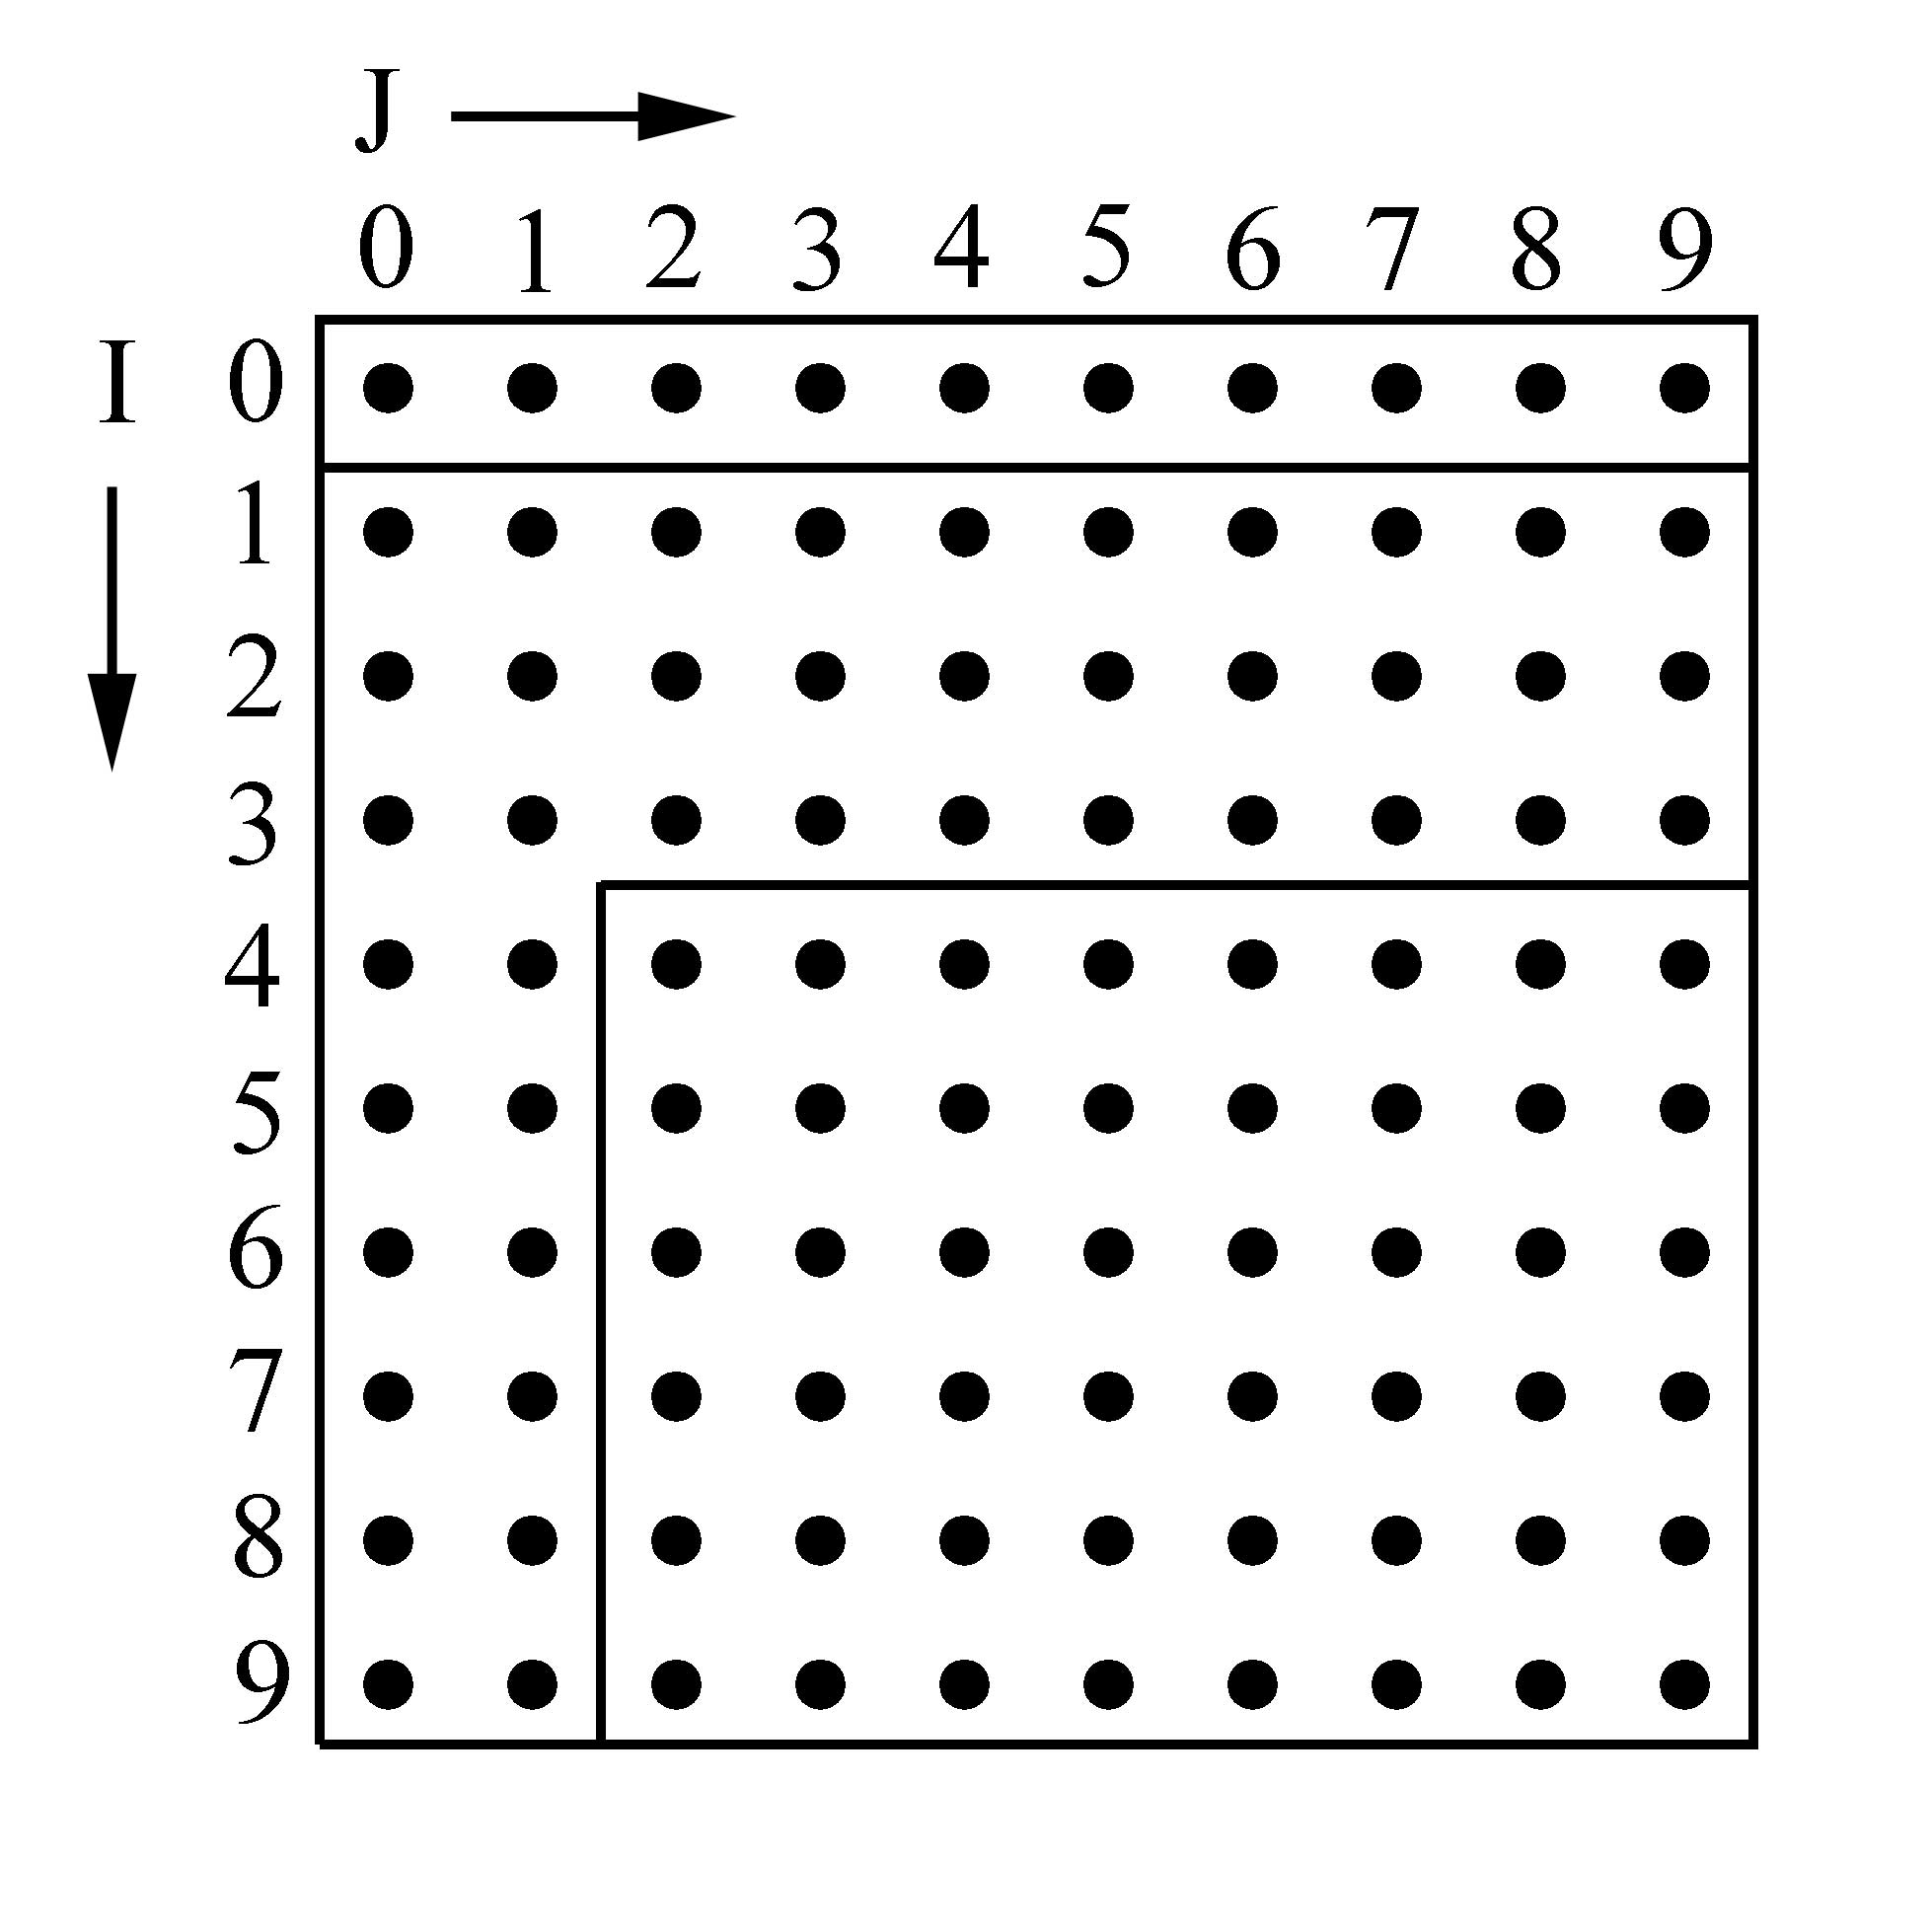
\includegraphics[width=0.5\textwidth]{Figures/variable_eg.jpg}
\end{figure}
\chapter{Analysis of Extended Cycle Shrinking Algorithm}

A dependence distance $\Phi(R)$ is called a dominating dependence distance if $\Phi(L) = \Phi(R)$. A dominating dependence distance may not always exist.  \\

The extended cycle shrinking algorithm is optimal only when there exists a dominating dependence distance. If cycle shrinking is applied to loops where this is not the case then it gives suboptimal partitions. \\

\noindent For example consider the following code: \\
DO I = 0, 9 \\
\indent DO J = 0, 9 \\
\indent \indent A[I+1, J+9] = B[I, J] \\
\indent \indent C[I+6, J+6] = A[I, J] \\
\indent \indent B[I+8, J+1] = C[I, J] \\
\indent ENDO \\
ENDO \\

The dependence distances are (1, 9), (6, 6) and (8, 1). $\Phi(L) = (1, 1)$. Thus, there is no dominating dependence distance in this case. The partitions created by extended cycle shrinking algorithm and a better possible partition is shown in Figure~\ref{fig:eg_opt}. This motivates us to optimize the extended cycle shrinking algorithm so to have optimal partitions even in those cases where there is no dominating dependence distance.\\

\begin{figure}
\centering
\begin{subfigure}{0.5\textwidth}
  \centering
  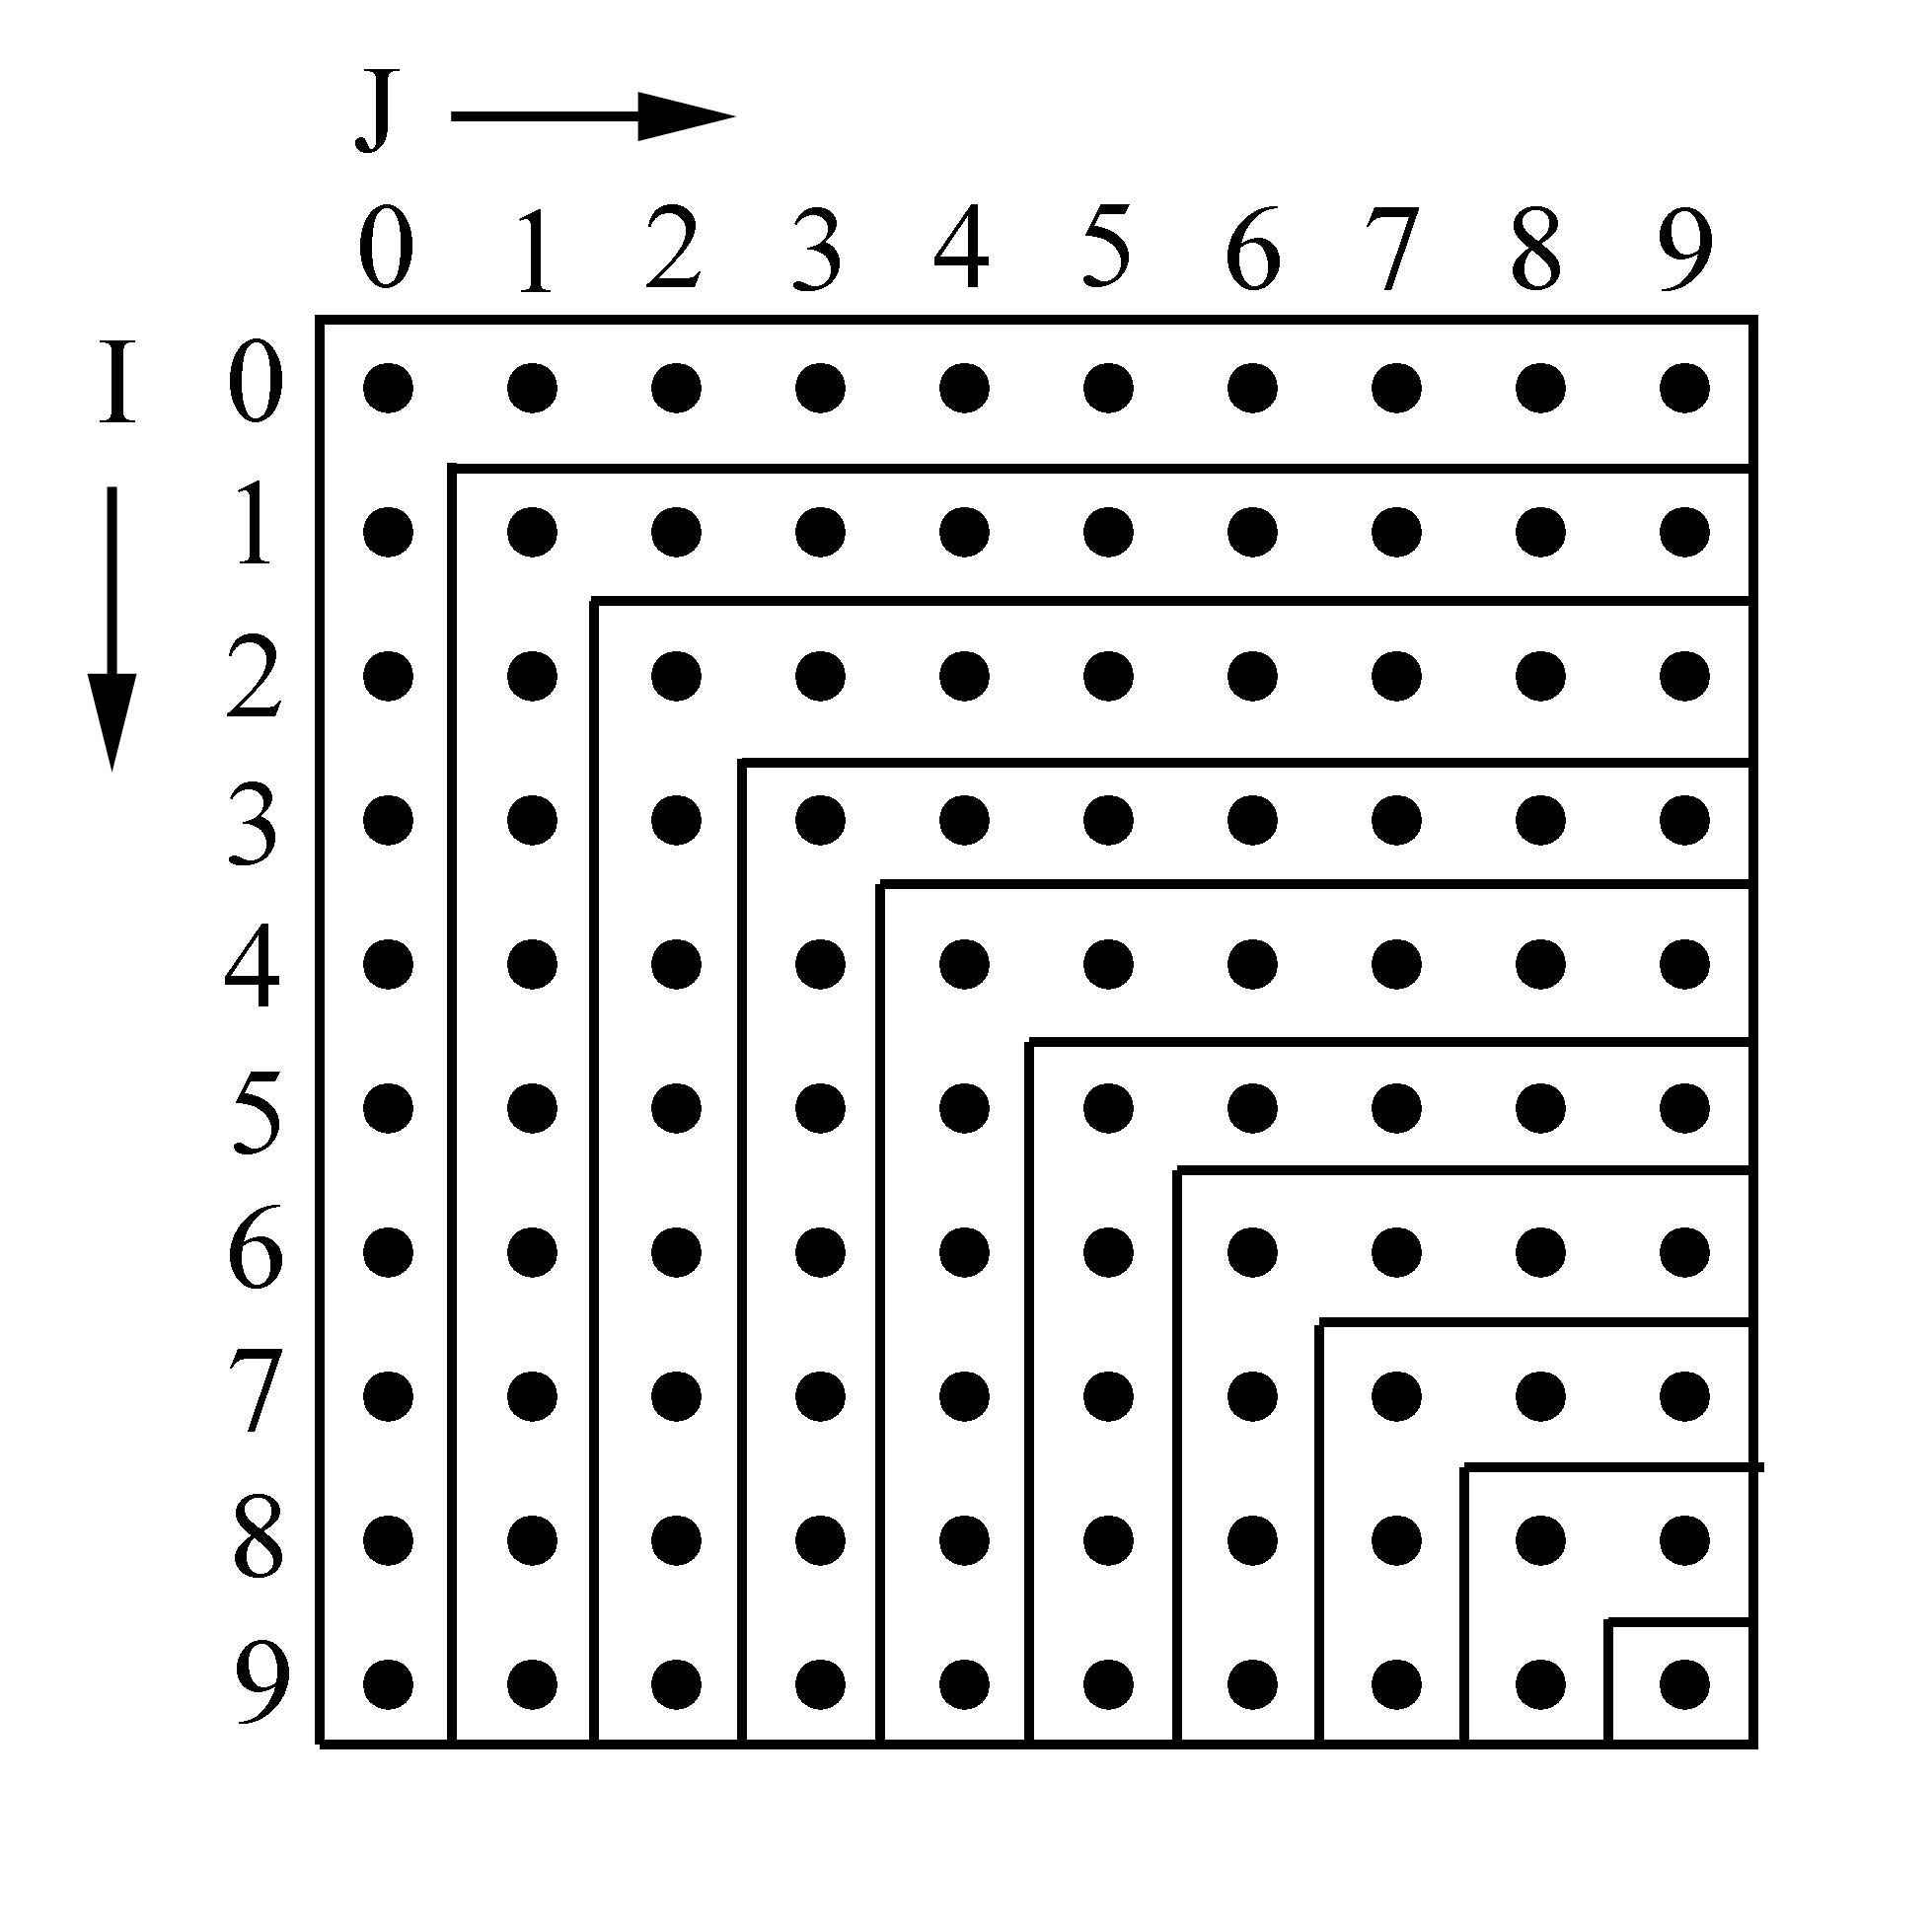
\includegraphics[width=\textwidth]{Figures/fig1a.jpg}
  \caption{}
  \label{fig:sub1}
\end{subfigure}%
\begin{subfigure}{0.5\textwidth}
  \centering
  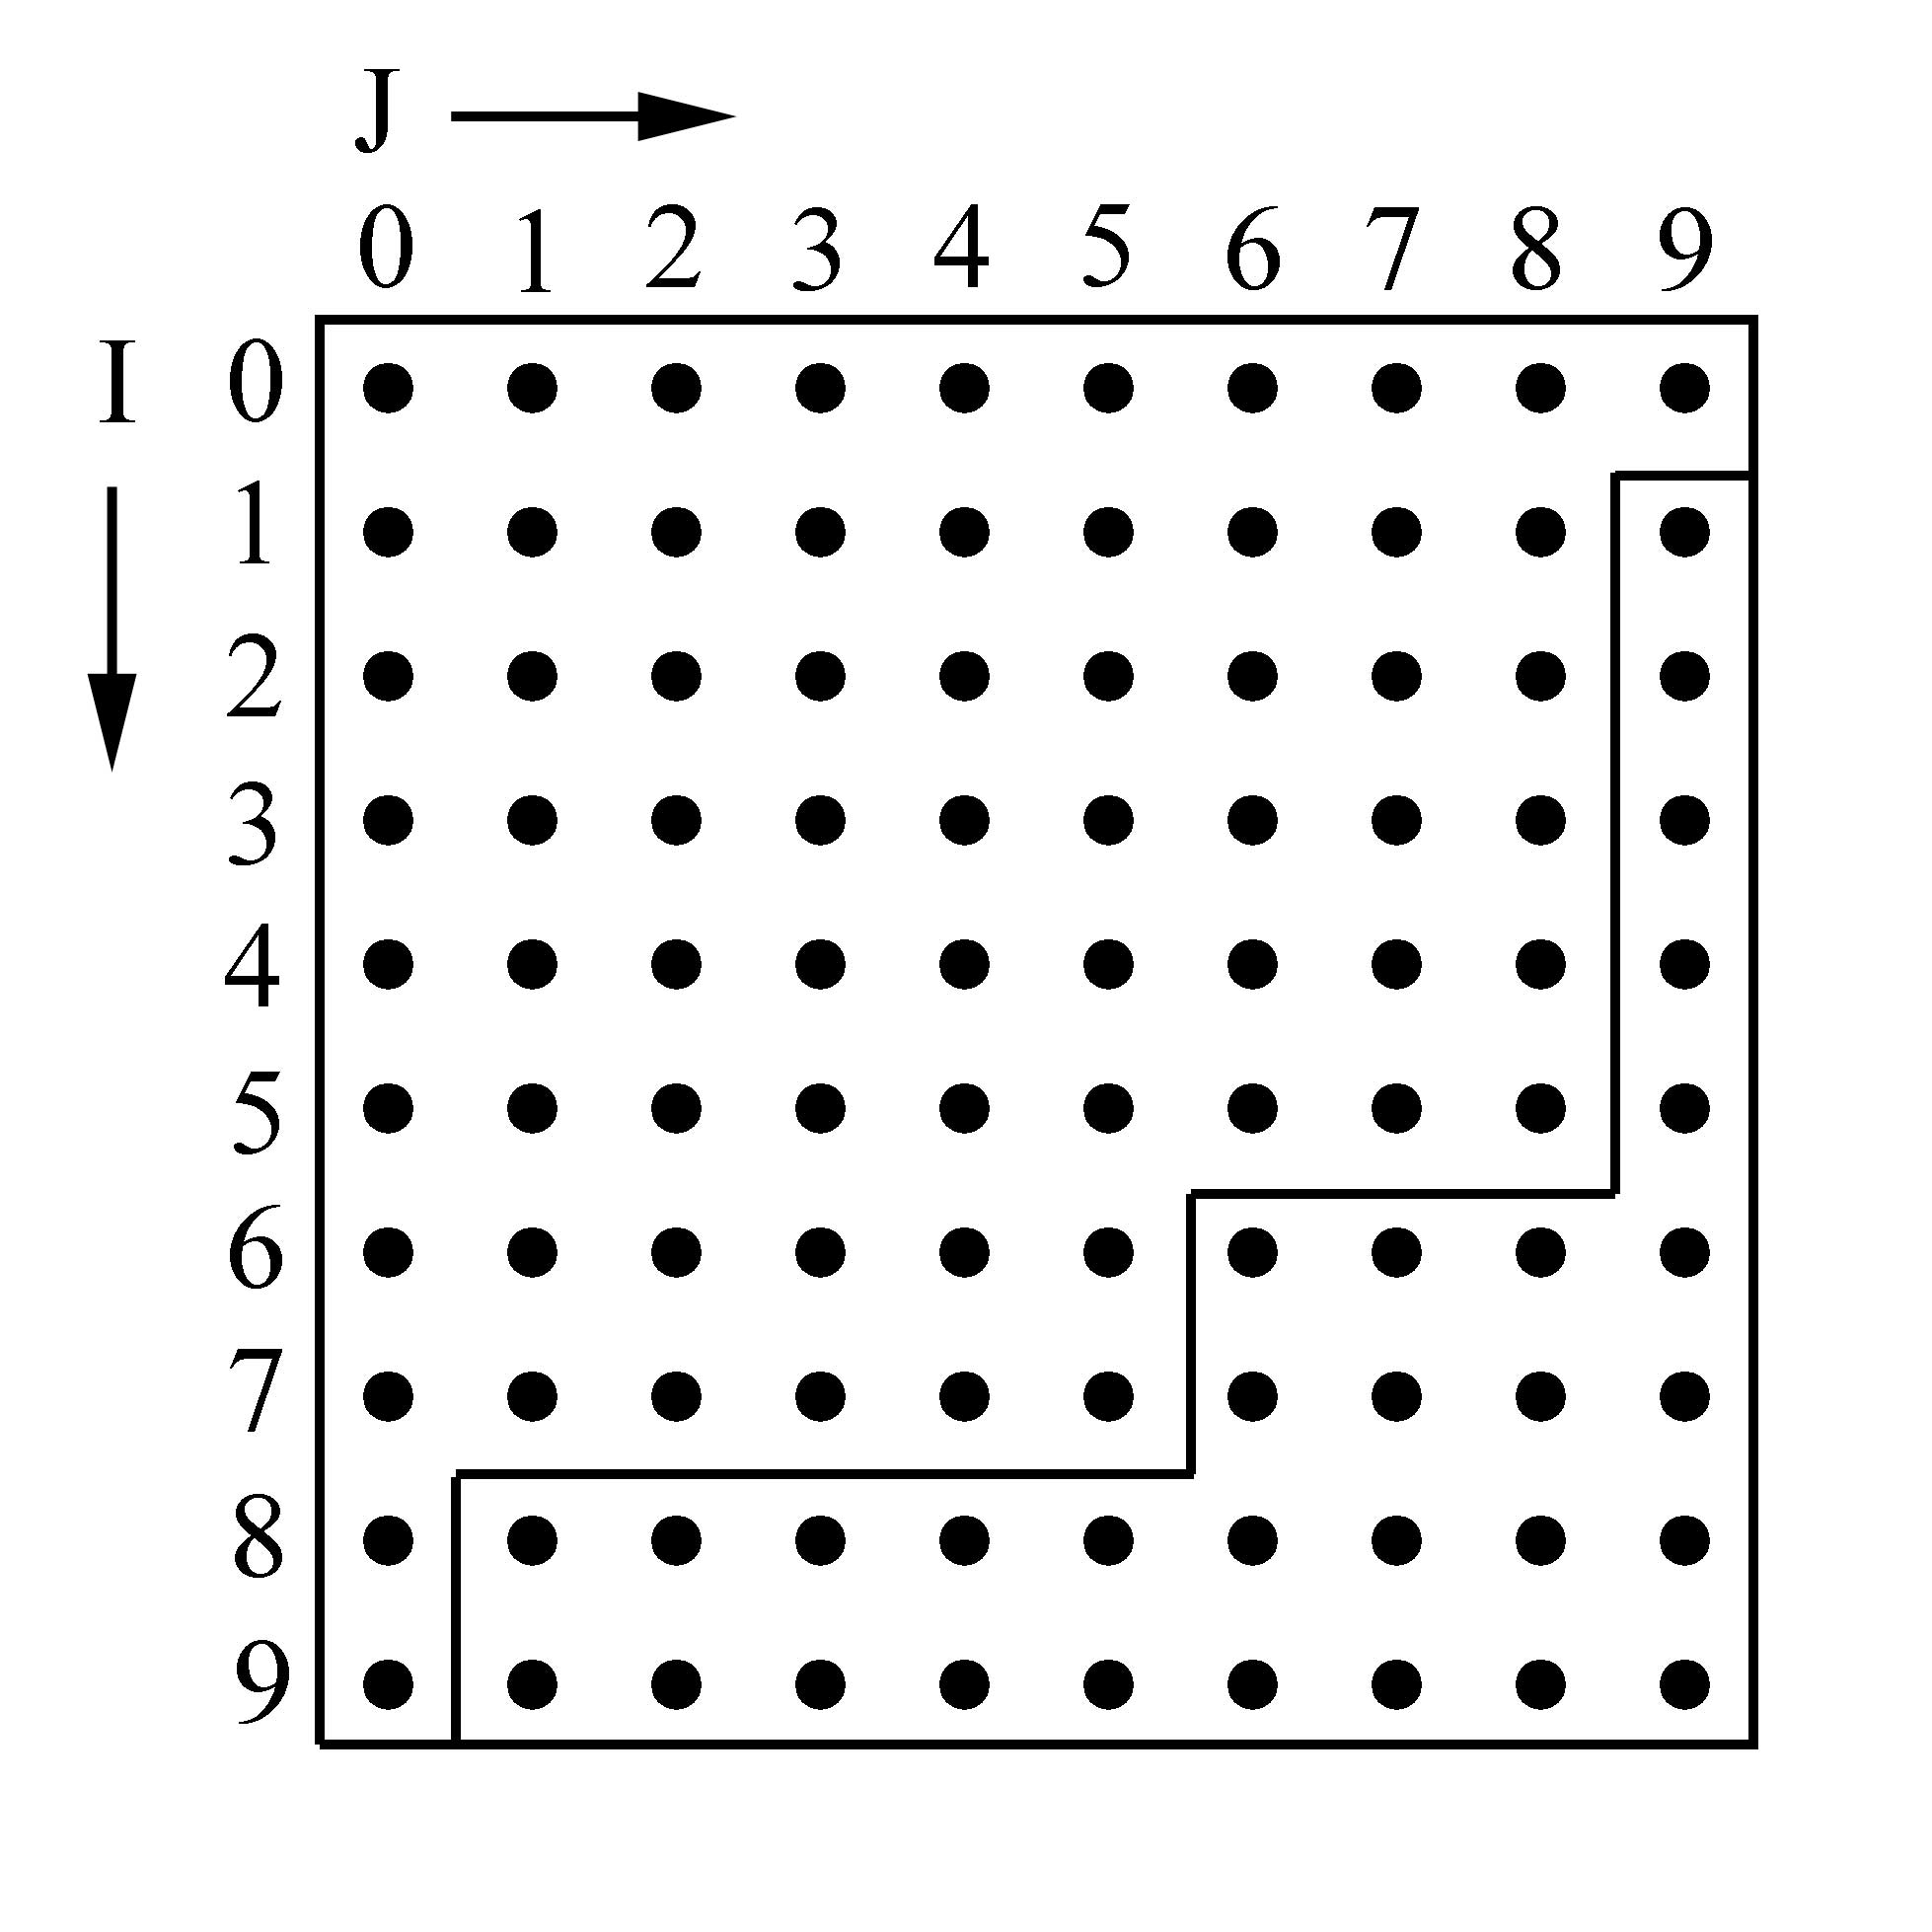
\includegraphics[width=\textwidth]{Figures/fig1b.jpg}
  \caption{}
  \label{fig:sub2}
\end{subfigure}
\caption{(a) Partitions by extended cycle shrinking algorithm. (b) Better partition}
\label{fig:eg_opt}
\end{figure}
\chapter{Our Algorithm}
We consider only those cases where all the dependence distances are positive. The algorithm can then be easily extended when all dependence distances are negative for a particular loop nest.
\section{Notation}
For a nested loop, the vector of loop index for each nest is called as an iteration point. For example, consider a doubly nested loop with outer loop index i and inner loop index j. Then iteration point a = (2, 3) means that at this point, i = 2 and j = 3. Also $a_1 = 2$, $a_2 = 3.$ \\

Iteration point a is said to dominate iteration point b if\\
 $ \forall k,  a_k \leq b_k$ \\
We denote it by $a \preceq b$.\\
This creates a partial order on the set of iteration points.\\

We denote a partition by two sets of points, set A and set B, belonging to the iteration space. This partition is represented by P(A,B). \\

P(A,B) is the set of all iteration points that are dominated by at least one iteration point in set A and are not dominated by any iteration point from set B \\
$P(A,B) = \{x | ( \exists a \in A, a \preceq x) and (\forall b \in B, not(b \preceq x))\}$ \\

Thus if we have sets $A_0, A_1, ... A_k$ then we have k partitions: \\
$P(A_0,A_1), P(A_1, A_2), P(A_2, A_3), ... , P(A_{k-1}, A_k)$. \\

\subsection{Example}

For the example in figure~\ref{fig:partition_eg}, the sets are as given below: \\
$A_0 = \{(0,0)\}$ \\
$A_1 = \{(1,4), (2,2), (3,1)\}$ \\
$A_2 = \{(2,8), (3,6), (4,4), (5,3), (6,2)\}$ \\
$A_3 = \{(5,8), (6,6), (7,5), (8,4), (9,3)\}$ \\
$A_4 = \{(8,8), (9,7)\}$ \\
$A_5 = \{\}$ \\

\begin{figure}
\caption{Partitions by our algorithm}
\label{fig:partition_eg}
\centering 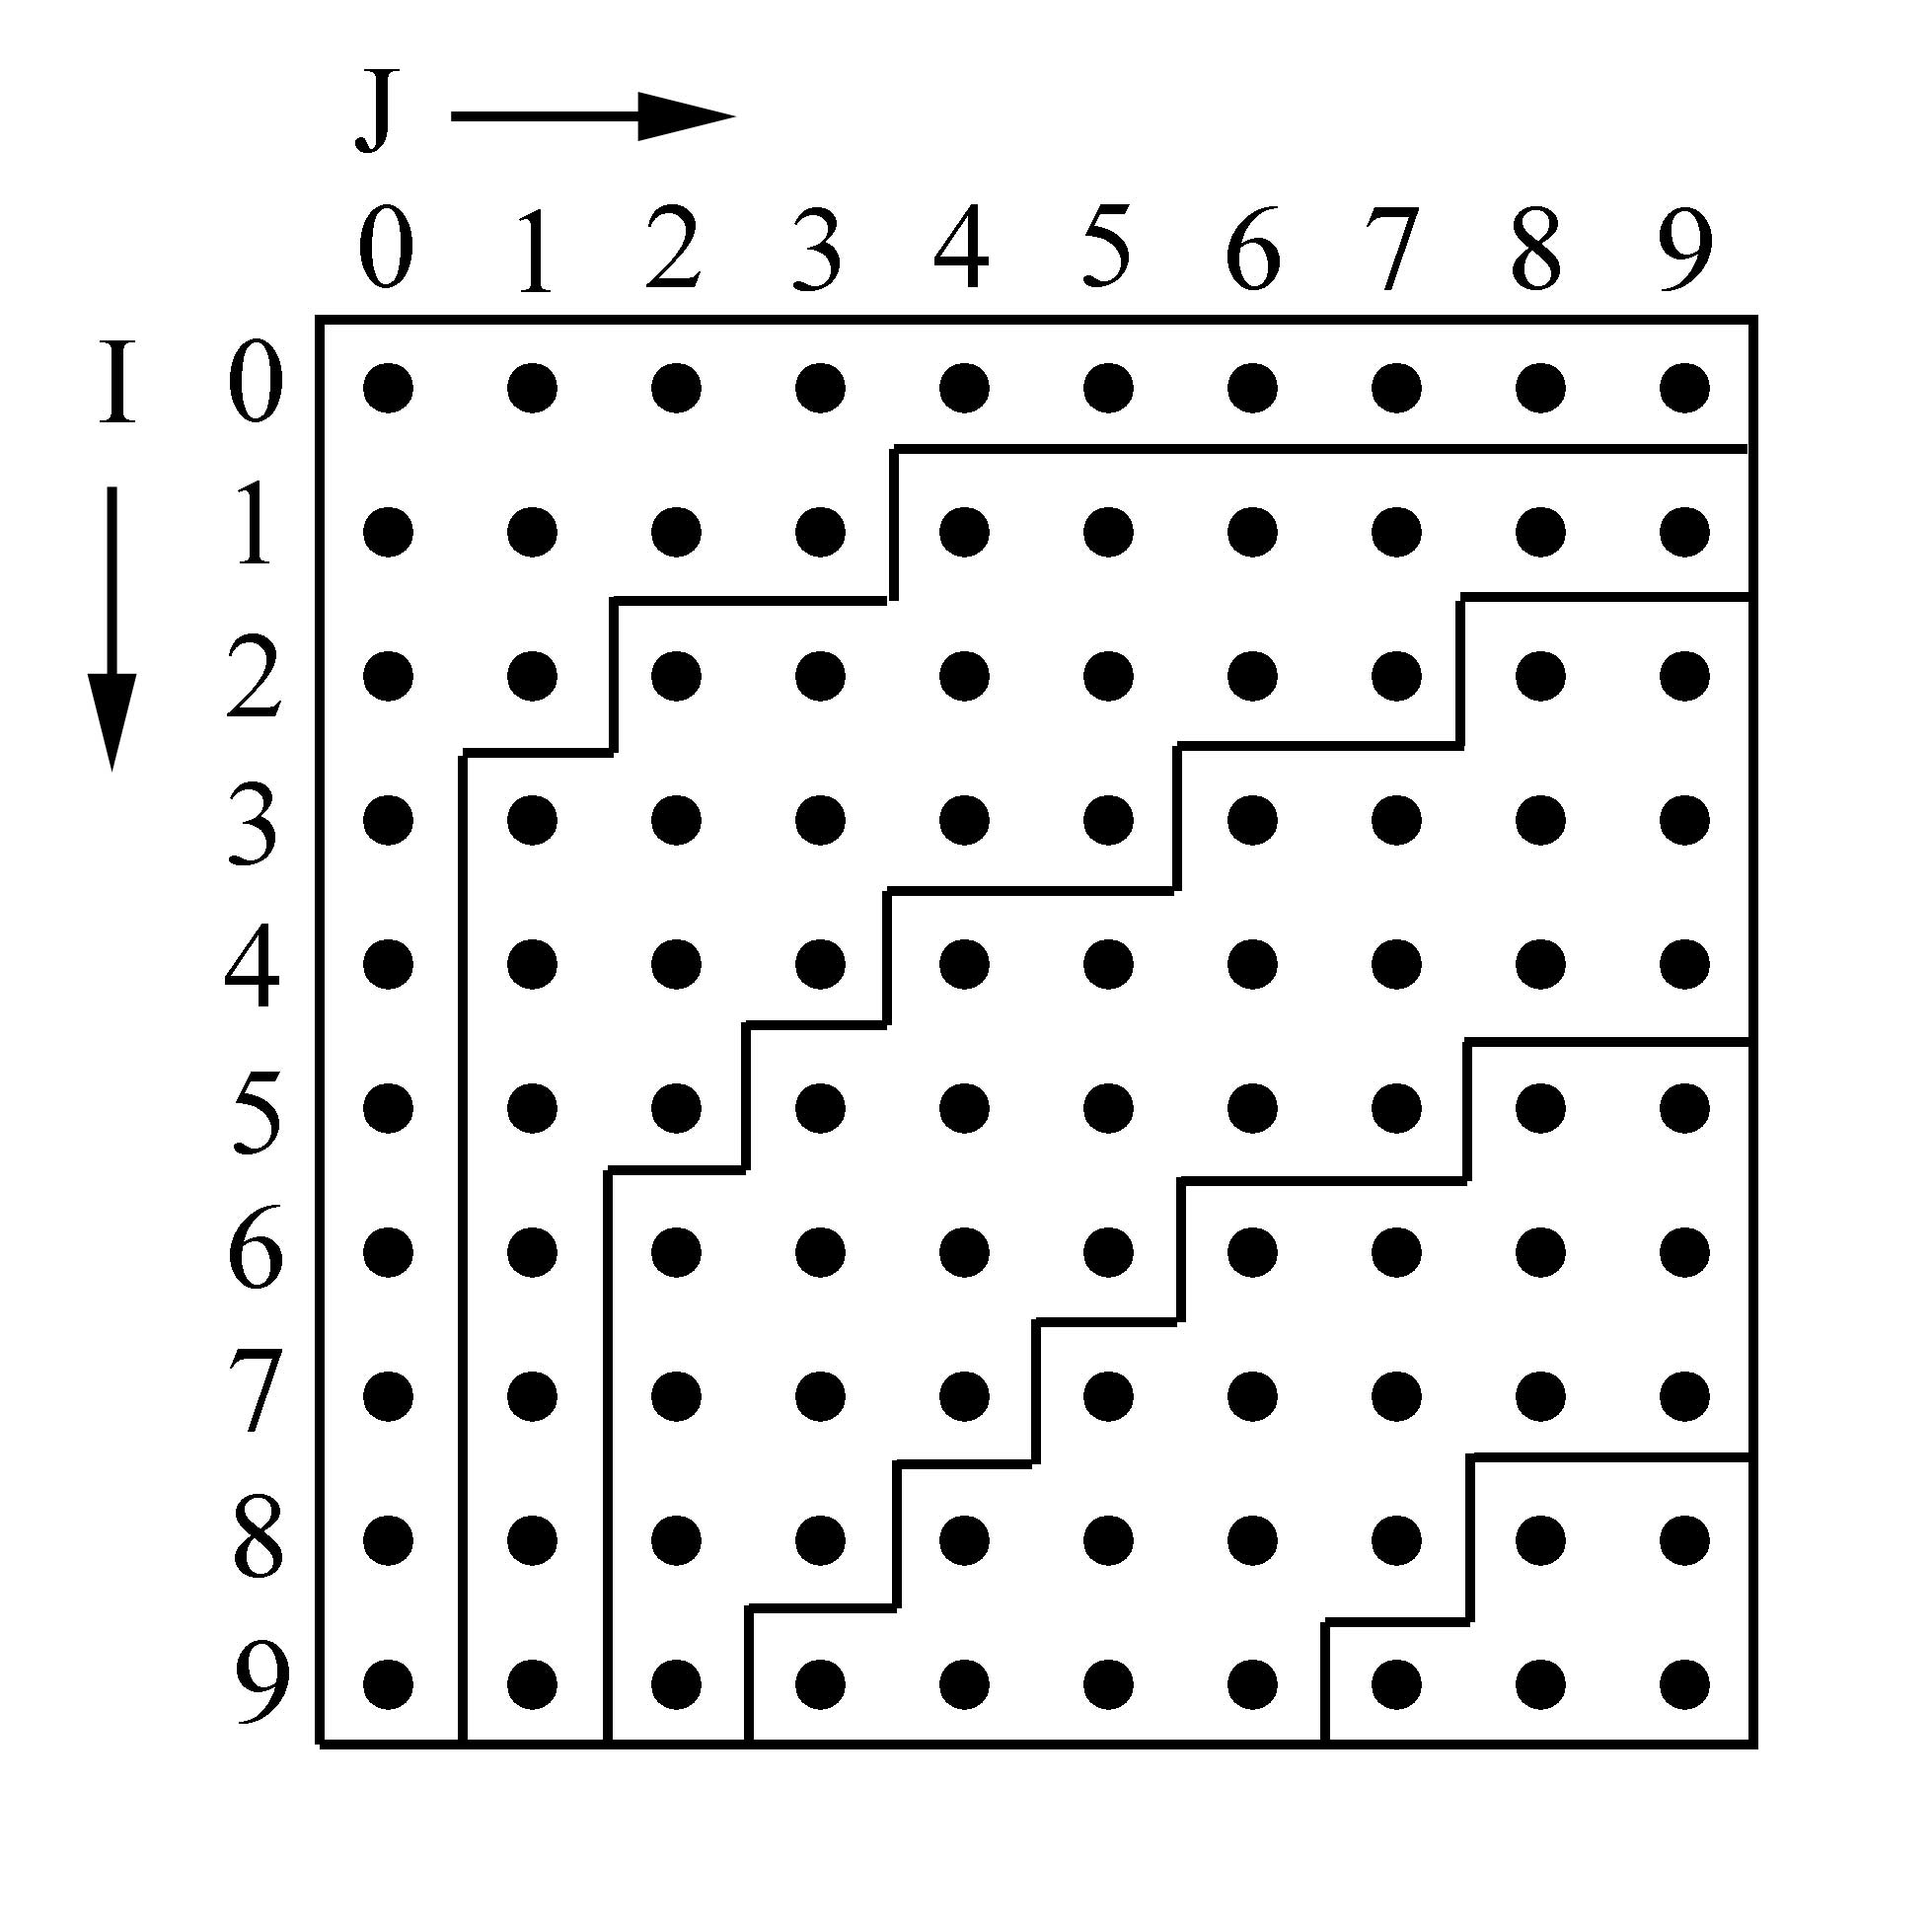
\includegraphics[width=0.5\textwidth]{Figures/fig2.jpg}
\end{figure}

%\ref{append:labelforappendix}

\section{Algorithm to generate the sets of points}

We give an iterative algorithm in which, given a set of points, it generates the next set.
Let the sets be called $A_0, A_1, .. ,A_k$ \\

Consider the set of all the dependence distances of the loop. 
Create a minimal set of dependence distances by removing any dependence distance that is dominated by another dependence distance in the set.
Thus in the minimal set, no dependence distance dominates any other dependence distance.
Call this set D. \\

\noindent
$A_0 = \{(0,0,..,0)\}$ /* Vector containing as many 0s as the total loop nest. First element corresponds to outermost loop and so on. */ \\
$iter = 0$ \\
while($A_{iter}$ is not empty) \{ \\
\indent	iter++ \\
\indent	$B = \{\}$ \\
\indent	$ \forall a \in A_{iter-1}, \forall d \in D$, insert a+d in B if a+d lies inside the loop bounds\\
\indent	Create a minimal set of B, by removing an iteration point from B if there exists another iteration point dominating it.\\
\indent	Thus in the final set obtained no iteration point dominates another point.\\
\indent	Set $A_{iter}$ as this minimal set obtained\\
\} \\

\subsection{Example}

\noindent For example consider the following code: \\
DO I = 0 to 9 \\
\indent DO J = 0 to 9 \\
\indent \indent A[I+1, J+4] = B[I, J] \\
\indent \indent C[I+2, J+2] = A[I, J] \\
\indent \indent B[I+3, J+1] = C[I, J] \\
\indent ENDO \\
ENDO \\

\noindent In this case, \\
$D = \{(1,4), (2,2), (3,1)\}$ \\
The above algorithm apllied to this example is shown in table~\ref{table:iterations}. \\
The partitions generated are depicted in figure~\ref{fig:partition_eg}. \\

\begin{table}
\caption {Iterations of the algorithm applied to example}
\label{table:iterations}
\begin{tabular}{|c| L{5.75cm} | L{5.75cm} | }

\hline

\bf iter &
\bf B &
\bf $A_{iter}$ \\ \hline

\bf 0 &
- &
$\{(0,0)\}$ \\ \hline

\bf 1 &
$\{(1,4), (2,2), (3,1)\}$ &
$\{((1,4), (2,2), (3,1)\}$ \\ \hline

\bf 2 &
$\{(2,8), (3,6), (4,5), (3,6), (4,4),$ $(5,3), (4,5), (5,3), (6,2)\}$ &
$\{(2,8), (3,6), (4,4), (5,3), (6,2)\}$ \\ \hline

\bf 3 &
$\{(5,9), (5,8), (6,7), (5,8), (6,6),$ $(7,5), (6,7), (7,5), (8,4), (7,6),$ $(8,4), (9,3)\}$ &
$\{(5,8), (6,6), (7,5), (8,4), (9,3)\}$ \\ \hline

\bf 4 &
$\{(8,9), (8,8), (9,7), (8,9), (9,7),$ $(9,8)\}$ &
$\{(8,8), (9,7)\}$ \\ \hline

\bf 5 &
$\{\}$ &
$\{\}$ \\ \hline

\end{tabular}
\end{table}

%\chapter{Proof of correctness and optimality}

\section{Correctness}
We need to prove that a source-sink pair can never lie in the same partition. We prove this by contradiction. \\

Suppose there exists a source u and sink v that lie in the same partition P(A,B).
Let the dependence distance between them be d.\\
Thus $v = u + d$\\
Consider $d' \preceq d$ and $d' \in D$\\

Lemma 1: There always exists such d'\\

\noindent Let $ v' = u + d'$\\
Thus, u, v' is another source-sink pair\\

Lemma 2: If $u, v \in P(A,B)$  then $u , v' \in P(A,B)$.\\

\noindent As, $u, v' \in P(A,B), \exists a \in A, a \preceq u$ \\
By the method in which partitions are created, \\
$\exists b \in B, b \preceq a + d'$ \\
$a \preceq u$ \\
$ \Rightarrow a + d' \preceq u + d'$ \\
$\Rightarrow b \preceq a + d' \preceq v'$ \\
$\Rightarrow b \preceq v'$ \\
Thus it implies v does not belong to P(A,B) which is a contradiction. \\

Thus, our assumption is false. Therefore there does not exist any source-sink pair belonging to same partition.\\

\subsection{Proof of Lemma 1}
If $d \in D$ then $d = d'$\\
else as d was removed from the set of dependence distances, there must exist another dependence distance in D dominating d. Let that be d' \\


\subsection{Proof of Lemma 2}
$u,v \in P(A,B)$ \\
$\Rightarrow \exists a \in A , a \preceq u$ \\
$ \Rightarrow a \preceq u \preceq v'$ \\
$ \Rightarrow a \preceq v' $ \\

Suppose $v' \notin P(A,B)$. \\
$ \Rightarrow \exists b \in B, b \preceq v'$ \\
$ d' \preceq d $ \\
$ \Rightarrow d' + u \preceq d + u $ \\
$ \Rightarrow v' \preceq v$ \\
$ (b \preceq v'$ and $v' \preceq v) \Rightarrow b \preceq v$ \\ 
$ \Rightarrow v \notin P(A, B)$ \\
Therefore our assumption is false. \\
$v' \in P(A,B)$ \\

\section{Optimality}
We need to prove that even if a single iteration point from a partition is added to its previous partition, it will lead to at least one source-sink pair belonging to same partition. \\

Suppose the partitions we created are not optimal. 
Therefore there exists a point y which is in the next partition of P(A,B) which can be added to P(A,B). i.e y has no source in P(A,B). \\

\noindent $y \notin P(A,B) \Rightarrow  \exists b \in B, b \preceq y$ \\
By the method in which partitions are created, \\
$ \exists d \in D$ and $a \in A, a + d = b$ \\
Let $x = y - d$ \\
$ b \preceq y \Rightarrow b - d \preceq y - d$ \\
$ \Rightarrow a \preceq x$ \\
This means that $x \in P(A,B)$ \\
x and y form a source-sink pair. Therefore there is a source of y in P(A,B).
Therefore our assumption is false. \\

Thus partitions created are optimal.\\
\chapter{Method to calculate the number of partitions}
We may need to find the number of partitions required in this algorithm without actually creating partitions so as to get an idea of how much parallelization is possible in the loop.
The method for that is given below. \\

Let the loop bounds be from 0 to $(n_i - 1)$ for loop nest i. \\
Let $d^1, d^2, ... , d^k$ be the elements of set D \\

The optimal value of the following integer linear optimization problem gives the number of partitions: \\

\noindent maximize $x_1 + x_2 + .. + x_k + 1$ \\
subject to \\
\indent $ \Sigma_{j=1}^{k} d_{i}^{j} * x_j  < n_i$ for each loop nest i \\
\indent $ x_j \geq 0$  $\forall j$ \\
\indent All $x_j$ are integral. \\ 

By giving the above linear optimization problem to a solver, the optimal value caluclated is the number of partitions required.


\subsection{Example}
Consider the same example,  \\
DO I = 0 to 9 \\
\indent DO J = 0 to 9 \\
\indent \indent A[I+1, J+4] = B[I, J] \\
\indent \indent C[I+2, J+2] = A[I, J] \\
\indent \indent B[I+3, J+1] = C[I, J] \\
\indent ENDO \\
ENDO \\

\noindent $d^1 = (1, 4)$ \\
$d^2 = (2, 2)$ \\
$d^3 = (3, 1)$ \\
$n_1 = 10$ \\
$n_2 = 10$ \\

The linear optimization problem for this case is: \\
maximize $x_1 + x_2 + x_3 + 1$ \\
subject to \\
\indent $ 1 * x_1 + 2 * x_2 + 3 * x_3 < 10 $ \\
\indent $ 4 * x_1 + 2 * x_2 + 1 * x_3 < 10 $ \\
\indent $ x_1 \geq 0 $ \\
\indent $ x_2 \geq 0 $ \\
\indent $ x_3 \geq 0 $ \\
\indent $x_1, x_2, x_3$ are integral. \\
\chapter{Loop Generation Algorithm}
We have given an algorithm to find the sets of points that can determine the optimal partitions. Now we give an algorithm to generate actual loops given these sets of points. \\

\section{Algorithm}


generate\_loop (A, B, boundaries, l) \{ \\

\noindent /* \\
generate\_loop takes two sets of points as input and outputs the loops representing P(A, B) \\

\noindent A, B are the sets of points representing partition P(A, B) \\
boundaries contains the upper limit of the index variables \\
l denotes the current loop nest level. \\
*/ \\

\indent	A = sort\_and\_dominate(A) \\
\indent	B = sort\_and\_dominate(B) \\

\indent	//BASE CASE \\
\indent	if A and B have points with only 1 dimension then \{ \\
\indent \indent		start = A.first()[0]; \\
\indent		if (B is empty) \{ \\
\indent\indent			end = boundarie[l]; \\
\indent		\} \\
\indent		else \{ \\
\indent\indent			end = B.first()[0] - 1; \\
\indent		\} \\
\indent		put forall $i_l$ = start to end \\
\indent		put all the statements to be executed \\
\indent		put endall \\

\indent		return; \\
\indent	\} \\
	
\indent	A' = empty \\
\indent	B' = empty \\
\indent	start = min (A.first()[0], B.first()) \\
	
\indent	while (A is not empty or B is not empty) \{ \\
		
\indent\indent		while (A.first()[0] == start) \{ \\
\indent\indent\indent			remove first point from A and put it in A' after removing the first dimension from it \\
\indent\indent\indent			// eg: if first point is (2, 4, 1), then put (4, 1) in A' \\
\indent\indent		\} \\
\indent\indent		while (B.first()[0] == start) \{ \\
\indent\indent\indent			remove first point from B and put it in B' after removing the first dimension from it \\
\indent\indent		\} \\

\indent\indent		if (both A and B are empty) \{ \\
\indent\indent\indent			end = boundaries[l]; \\
\indent\indent		\} \\
\indent\indent		else \{ \\
\indent\indent\indent			end = min(A.first()[0], B.first()[0]) - 1; \\
\indent\indent		\} \\

\indent\indent		put forall $i_l$ = start to end \\
\indent\indent		generate\_loop (A', B', boundaries, l+1); \\
\indent\indent		put endall \\

\indent\indent		start = end + 1 \\
\indent	\} \\
\} \\	

sort\_and\_dominate() sorts all the points on the first dimension and also removes redundant points, i.e., if a,b belongs A and a <= b then b is removed from A.


\include{Chapters/variable_dependence_distance}
\include{Chapters/negative_distances}
\include{Chapters/parallelizing_algorithm}
\chapter{Future Work}
We have given an algorithm to find the sets of points that can determine the optimal partitions. We have also implemented the algorithm to generate these sets. But the task of actually creating the partitions in the form of loops is yet to be done. This should be the next step which will complete this algorithm. \\

After this, the complete algorithm can be implemented. A testing platform can be created and the algorithm can be put to test so as to have performance analysis of the algorithm. \\

We have given an optimal algorithm for constant dependence distance case. But there is a lot to be done in variable dependence distance case. Similar idea can be applied in variable distance case also to get improvement. \\
\pagenumbering{roman}
%\appendix
\chapter{Title of first appendix}
\section{First Section}
\label{append:labelforappendix}
Here's how you write code.
\begin{verbatim}
#include <stdio.h>

main()
{
    printf("hello, world\n");
}
\end{verbatim}

\section{Second Section}
Here's how you write installation instructions.
\begin{verbatim}
$ cd /home/username/documents
$ git clone https://github.com/mindprince/btp-report-latex-template.git
\end{verbatim}
\printbibliography[heading=bibintoc]

\end{document}